%!TEX TS-program = xelatex
%!TEX encoding = UTF-8 Unicode

% Um dieses Dokument zu erzeugen sind folgende Pakete erforderlich:
% - texlive-xetex (oft aber nicht immer Teil der TexLive-Distribution)
% - texlive-lang-german (auch nicht immer dabei)
% - Möglicherweise mehr TexLive-Pakete (siehe Logdatei nach dem Kompilieren).
% - Die Schrift "Linux Libertine".
% - Das Paket "libertine.sty". Achtung, nicht mit dem gleichnamigen LaTeX-Paket
%		verwechseln, welches unglücklicherweise standardmässig auch von XeTeX
%		gezogen wird. Es genügt das mitgelieferte Paket im gleichen Ordner
%		wie das Tex-Dokument bereitzustellen.
% - Die Schrift "Liberation Mono"
% - Das FHNW-Logo "fhnw-technik-head.eps"
%
% Das Dokument wird erzeugt mit: $ xelatex Report.tex
% Aufgrund der Querverweise sind nach Änderungen jeweils zwei xelatex-Läufe nötig.
%
\documentclass[paper=A4,twoside=false,BCOR=0mm,DIV=calc,fontsize=12pt,enabledeprecatedfontcommands]{scrartcl}
%
\usepackage[automark,headsepline]{scrpage2}
\usepackage{xunicode,fontspec,xltxtra}
\usepackage[english,german]{babel}
\usepackage{graphicx}
\usepackage{lastpage}
\usepackage[pagebackref=true,colorlinks=true,allcolors=black]{hyperref}
\usepackage{listings}
\usepackage{csquotes}
%
\usepackage{enumitem}
\setlist[itemize]{noitemsep}
%
% Beautiful tables
\usepackage{booktabs}
\newcommand{\ra}[1]{\renewcommand{\arraystretch}{#1}} % Set on every table the space
%
% Graphs
\usepackage{pgf}
\usepackage{tikz}
\usetikzlibrary{arrows}
\usepackage{smartdiagram}
\usepackage{color}
\usepackage{xcolor}
%
\usepackage{pdfpages}
\usepackage{rotating}
%
\usepackage{pgfplots}
\usepgfplotslibrary{ternary}
\pgfplotsset{compat=1.8}
%
\usepackage{mathtools}
%\everymath{\displaystyle} use $\displaystyle \sum$ in text
\usepackage{amstext}
\renewcommand{\listfigurename}{Abbildungen}
%
% fuer Zitate
\usepackage{cite}
%\bibliographystyle{alphadin}
%\usepackage[debug]{libertine}
%\setromanfont[Mapping=tex-text]{Linux Libertine O}
%\setsansfont[Mapping=tex-text]{Linux Biolinum O}
%\setmonofont[Mapping=tex-text]{Liberation Mono}

\pagestyle{scrheadings}
\clearscrheadfoot{}
\ihead{\headmark}
%\ohead{Seite\pagemark\ von \pageref{LastPage}}
%\ifoot{P. Steinger \& N. Mauchle}
%\ofoot{\today}
\ofoot{Seite\pagemark\ von \pageref{LastPage}}

% Two images beside
\usepackage{subcaption}
%
%
\setlength{\parindent}{0pt}
\setlength{\parskip}{1em}
%
\newenvironment{myenumerate}{
\begin{enumerate}
  \setlength{\itemsep}{0pt}
  \setlength{\parskip}{0pt}
}{\end{enumerate}}
%
\newenvironment{myitemize}{
\begin{itemize}
  \setlength{\itemsep}{0pt}
  \setlength{\parskip}{0pt}
}{\end{myitemize}}
%
\renewcommand*{\pnumfont}{
	\normalfont\rmfamily\slshape
}
%
\KOMAoptions{draft=true}
\KOMAoptions{DIV=last}
%
\textheight=630pt
%
%\usepackage{layout}
\begin{document}
\overfullrule=0pt
%
\definecolor{lightgray}{rgb}{.9,.9,.9}
\definecolor{darkgray}{rgb}{.4,.4,.4}
\definecolor{purple}{rgb}{0.65, 0.12, 0.82}
%
\lstdefinelanguage{Python}{
  keywords={typeof, new, True, False, except, function, return, null, catch, switch, var, if, in, while, do, else, case, break},
  keywordstyle=\color{blue}\bfseries,
  ndkeywords={class, export, boolean, throw, implements, import, this},
  ndkeywordstyle=\color{darkgray}\bfseries,
  identifierstyle=\color{black},
  sensitive=false,
  comment=[l]{//},
  morecomment=[s]{/*}{*/},
  commentstyle=\color{purple}\ttfamily,
  stringstyle=\color{red}\ttfamily,
  morestring=[b]',
  morestring=[b]"
}
%
\lstset{
   language=Python,
   backgroundcolor=\color{lightgray},
   extendedchars=true,
   basicstyle=\footnotesize\ttfamily,
   showstringspaces=false,
   showspaces=false,
   numbers=left,
   numberstyle=\footnotesize,
   numbersep=9pt,
   tabsize=2,
   breaklines=true,
   showtabs=false,
   captionpos=b
}
%
%\layout
%
% --- Titelseite --- %
\begin{titlepage}
	\enlargethispage{3cm}
	\begin{raggedright}
	\begin{picture}(0,0)
		\put(-30,14){
\includegraphics[width=7cm]{fhnw-technik-head}}
	\end{picture}

	\vspace*{4cm}
	{\Huge\bfseries\normalfont\sffamily
		Mit Machine Learning Immobilienpreise schätzen\\[1.7ex]
	}
	{\Large\bfseries\normalfont\sffamily
		Vergleich von verschiedenen Machine Learning Algorithmen um Immobilienpreise zu schätzen.\\[2.2ex]
	}
	{\large\bfseries\normalfont\sffamily
		Projekt 6 von\\[1.5ex]
		Piero Steinger\\[1.5ex]
		Nicolas Mauchle\\[1.5ex]
	}
	\vspace*{1.5cm}
	{\large\bfseries\normalfont\sffamily
		FHNW\\[1.5ex]
		Hochschule für Technik\\[1.5ex]
		Studiengang IT\\[2.5ex]

		Examinator:\\[1.5ex]
		Prof. Dr. Manfred Vogel\\[2.5ex]

		Experte:\\[1.5ex]
		Johanes Schwertfeger\\[1.5ex]
	}
	\vspace*{2cm}
	{\large\bfseries\normalfont\sffamily
		Windisch, \today\\
	}
	\end{raggedright}
\end{titlepage}
%
\newpage
%
\pagenumbering{Roman}
% --- Zusammenfassung --- %
\section*{Abstract}
Häuserpreise werden heute von Experten geschätzt. Dafür muss ein Experte das Haus begutachten und diverse Kennwerte aufnehmen. Das kostet Geld und ist für beide Parteien mit Aufwand verbunden. Zudem weichen Schätzungen von verschiedenen Maklern zum Teil stark voneinander ab.

In diesem Projekt wird analysiert, ob ein Machine Learning Ansatz ähnliche oder sogar bessere Schätzungen abgeben kann. Zu diesem Zweck werden Immobiliendaten direkt aus dem Internet gesammelt und analysiert. Anhand von verschiedenen Machine Learning Algorithmen wird versucht ein exaktes Schätzungsmodell zu berechnen.

% --- Vorwort ----------------------------------------------------- %
\section*{Vorwort}
Das Projekt \emph{Mit Machine Learning Immobilienpreise schätzen} ist eine Forschungsarbeit im Rahmen der Bachelor Arbeit. Es soll untersucht werden, ob öffentliche Immobiliendaten ausreichen um akkurate Schätzungsmodelle zu erstellen.

Die Autoren bedanken sich bei Prof. Dr. Manfred Vogel, er hat das Projekt betreut und unterstützt.


%
% --- Inhaltsverzeichnis --- %
\newpage
	\tableofcontents
%
\clearpage
\pagenumbering{arabic}
\newpage
%
% --- Einleitung --- %
\section{Problemstellung}
Machine Learning wird heute in sehr vielen Gebieten eingesetzt \cite{forbes}. Das Schätzen eines Kaufpreises einer Immobilie ist ein klassischer Anwendungsfall. Der Grund dafür sind die vielen Kennwerte, die eine Immobilie besitzt.\\
Heute werden Immobilienpreise\footnote{Der Verkehrswert einer Immobilie.} immer noch von Experten geschätzt. Dies obwohl Machine Learning Algorithmen in der Lage sind eine gleichwertige oder sogar präzisere  Schätzung abzugeben.\\
Damit ein gutes Schätzungsmodell berechnet werden kann, braucht es einen aussagekräftigen Datensatz. Einen solchen Datensatz mit genügend Daten zu erstellen ist nicht trivial und kostet viel Zeit. Ausserdem existiert noch kein öffentlich zugänglicher Datensatz für den Schweizer Immobilienmarkt.\\
Für die Beschaffung der Immobiliendaten in der Schweiz bieten sich daher die vielen Immobilienplattformen im Internet an. Leider sind diese Daten stellenweise unvollständig oder fehlerhaft erfasst. Auch können Immobilien über zwei oder mehrere Plattformen beworben werden.\\
Es ist daher interessant zu wissen, ob mit öffentlichen Daten einen Datensatz erstellt werden kann, der mit aktuellen Machine Learning Algorithmen den Immobilienpreis akkurat schätzt. Zudem wäre dies auch für Makler und Immobilienbesitzer attraktiv, da sie diese Schätzungen als Unterstützung verwenden können.
%
\subsection{Ausgangslage}
In der Schweiz konkurrieren dutzende Immobilienplattformen im Internet, auf denen Immobilien zum Kauf oder Miete ausgeschrieben sind. Täglich kommen neue Inserate hinzu. Diese Daten stehen jedem frei zur Verfügung. Sie sind jedoch von Plattform zu Plattform unterschiedlich erfasst und müssen für die weitere Verwendung harmonisiert werden. Darüber hinaus müssen fehlerhafte oder doppelte Inserate erkannt und entfernt werden. Ferner können ortsbezogene Informationen vom Bundesamt für Statistik (BFS) eingeholt werden, um ein Inserat mit zusätzlichen Informationen zu ergänzen. Die Daten vom BFS stehen ebenso öffentlich zur Verfügung.

Zum Thema \textit{Kaufpreise für Immobilien schätzen} wurden diverse Forschungsarbeiten veröffentlicht \cite{existing_work_1, existing_work_2, existing_work_4}.
Nicht immer ist der einzelne Kaufpreis einer Immobilie gefragt, sondern mehr die Entwicklung des Immobilienpreises für eine spezifische Ortschaft \cite{existing_work_5}. Ähnliche Forschungsarbeiten wurden auch für die Schweiz durchgeführt. Meist wird jedoch versucht den Mietpreis pro Quadratmeter und nicht den Kaufpreis zu schätzen \cite{existing_work_3, existing_work_6}.
%
\subsection{Hypothese und Forschungsfragen}
In dieser Arbeit soll erforscht werden, ob mit öffentlich zugänglichen Immobilieninseraten und Machine Learning Algorithmen der Kaufpreis einer Immobilie akkurat geschätzt werden kann.\\
Zusätzlich zu den Immobilieninseraten werden geobasierte Daten vom Bundesamt für Statistik hinzugezogen um zu überprüfen, ob eine präzisere Schätzung erzielt werden kann.

Um den Kaufpreis einer Immobilie zu bestimmen, können verschiedene Verfahren angewendet werden. Diese Verfahren entsprechen keiner exakten Wissenschaft. Unter anderem auch deshalb, weil der Kaufpreis stark von Angebot und Nachfrage abhängig ist. Experten auf dem Gebiet sprechen von einem wirtschaftlich verkraftbaren Preis. Somit unterliegen die Preise einer gewissen Schwankung. Bei einer Experteneinschätzung wird von einer übereinstimmenden Bewertung gesprochen, wenn die Schätzwerte nicht mehr als 10\% voneinander abweichen \cite{immo_1, immo_2}.\\[2ex]
%
Für die Arbeit wird folgende These aufgestellt:\\[2ex]
\textit{Anhand von öffentlich gesammelten Daten können drei Viertel aller Immobilienpreise mithilfe von Machine Learning Algorithmen mit einer maximalen Abweichung von 10\% geschätzt werden.}\\[4ex]
%
Um diese These zu beantworten, werden folgende Forschungsfragen untersucht:
\begin{enumerate}
\item Wie gut reichen öffentliche Immobiliendaten aus, um aussagekräftige Daten zu erhalten?
\item Wie stark kann das Resultat verbessert werden, wenn geobasierte Daten hinzugefügt werden?
\item Welche Machine Learning Algorithmen eignen sich am Besten, um Immobilienpreise zu schätzen?
\end{enumerate}
Als Endergebnis soll eine Softwareapplikation aufzeigen, wie genau der Immobilienpreis geschätzt werden kann. Dazu werden diverse Algorithmen mit verschiedenen Parametern untersucht. Dabei kann nicht ausgeschlossen werden, dass noch exaktere Varianten oder Algorithmen vorhanden sind, die ein genaueres Resultat erzielen.
%
\subsection{Methode}
Für diese Arbeit wird mit dem iterativen Vorgehensmodell Plan Do Check Act (PDCA) gearbeitet. Dies erlaubt nach jeder Iteration das Resultat zu analysieren und, wenn möglich, in einer weiteren Iteration zu verbessern. Dazu ist es flexibel genug, um auf Fehlentscheide schnell reagieren zu können.
%
\subsection{Struktur}
Im nächsten Kapitel werden die verwendeten Machine Learning Algorithmen vorgestellt. Darauffolgend wird die Architektur aufgezeigt. Im Kapitel Validierung werden die gesammelten Daten ausgewertet und die Machine Learning Algorithmen untersucht, um die Studienfrage zu beantworten. Im letzten Kapitel findet sich ein Résumé der Arbeit.
\newpage
%
\section{Hintergrund}
In diesem Kapitel wird auf die Konzepte und Begriffe von Webcrawlern und Machine Learning eingegangen. Es soll ein gemeinsames Grundwissen für beide Gebiete geschaffen werden.
%
\subsection{Webcrawler}
Um Informationen von Webseiten zu sammeln, muss deren Inhalt analysiert und die gewünschten Daten extrahiert werden. Für diese Aufgabe eignen sich Webcrawler besonders gut \cite{scrapy_1, scrapy_2}.\\
Dabei erhält ein Webcrawler eine oder mehrere Einstiegs-URLs. Diese werden dann vom Crawler aufgerufen und die dazugehörigen Seiten ausgewertet. Bei der Auswertung kann der Crawler auf weitere URLs stossen, die er in seine Liste der abzuarbeitenden URLs aufnehmen kann. Sind alle URLs abgearbeitet ist der Crawler fertig. Je nach Aufgabenbereich existieren verschiedene Crawler-Techniken.\\
Ist bekannt von welchen Seiten die Informationen gecrawlt werden können, eignet sich am besten ein fokussierter Crawler. Dieser Crawler steuert vordefinierte Seiten an und extrahiert Informationen nach vorgegebenen Regeln.\\
Sind die Webseiten nicht bekannt oder haben die gesuchten Informationen keine definierte Struktur, eignen sich Deep Web Crawler. Diese bewegen sich mehrheitlich autonom und versuchen durch analysieren des Inhaltes herauszufinden, ob der Inhalt von Interesse ist oder nicht.\\
Sind übermässig viele Seiten zu crawlen, oder ist die Stabilität der Crawler wichtig, kommen verteilte Crawler zum Einsatz. Durch die Verteilung wird an Stabilität gewonnen und die Last auf die verschiedenen Crawler verteilt \cite{scrapy_3}.\\[2ex]
%
Um Daten von einer Webseite zu extrahieren, gibt es diverse Möglichkeiten. Von der einfachen Stringsuche bis zu Machine Learning Methoden kann nahezu alles angewendet werden. Beim fokussierten Crawlen wird häufig versucht Informationen über den XPATH oder über die CSS-Klassen zu extrahieren. Beide Varianten haben ihre Vor- und Nachteile, sind aber im Grunde sehr ähnlich \cite{xpath_vs_css}. Somit ist es dem Benutzer überlassen welche Variante er wählt \cite{xpath}.\\[2ex]
%
Eine Herausforderung beim Crawlen ist, dass der Crawler nicht als solchen vom Webseitenbetreiber erkannt wird. Diverse Betreiber möchten gerne verhindern, dass Informationen von Ihren Seiten gecrawlt werden \cite{comparis}.\\
Ist ein Crawler zu aggressiv, kann es vorkommen, dass er vom Betreiber gesperrt wird. Es gilt daher mit einer gewissen Raffinesse vorzugehen. Um möglichst nicht aufzufallen, ist es sinnvoll nur ein paar Requests\footnote{Anfrage auf eine Webseite} pro Minute abzusetzen und einen existierenden User Agent String\footnote{Browser/Crawler Kennung für die Website} anzugeben. Wenn das nicht ausreichend ist, können die Seiten über einen Pool von rotierenden IP-Adressen aufgerufen werden. So ist die Quelladresse nicht immer dieselbe \cite{offensive_crawling}.
%
\subsection{Machine Learning}
Machine Learning ist eine Art Künstliche Intelligenz (AI), das Softwareapplikationen erlaubt Vorhersagen anhand von trainierten Algorithmen zu erstellen.
Die Definition von Machine Learning aus dem Jahr 1959 von Arthur Samuel, einer der Pioniere im Bereich Machine Learning, lautet \cite{what_is_ml}:
  \begin{quote}
  \textit{Machine Learning: Field of study that gives computers the ability to learn without being explicitly programmed.}
  \end{quote}
Mit Hilfe von Machine Learning Algorithmen können neben Vorhersagen auch Trends erkannt oder Klassifizierungen durchgeführt werden \cite{ml_book}.
Dabei handelt es sich nicht um eine exakte Wissenschaft. Es lohnt sich verschiedene Algorithmen mit unterschiedlichen Parametern auszuprobieren, um die beste Performance zu finden. Vieles hängt auch von den Ausgangsdaten ab \cite{ml_azure}.

Grundsätzlich erhält ein Algorithmus Daten, die er zu einem Modell verarbeitet. Dieses Modell wird ausgewertet. Entspricht es nicht den gewünschten Anforderungen wird versucht ein besseres Modell zu erstellen, bis das Resultat zufriedenstellend ist. Abbildung \ref{fig:ml_process} zeigt den schematischen Ablauf.\\
\begin{figure}[ht]
\centering
\begin{tikzpicture}[
  font=\sffamily,
  every matrix/.style={ampersand replacement=\&,column sep=1.5cm,row sep=.5cm},
  source/.style={draw,thick,rounded corners,fill=yellow!20,inner sep=.3cm},
  process2/.style={draw,thick,rounded corners,fill=blue!20,inner sep=.3cm},
  process/.style={draw,thick,circle,fill=orange!20},
  process3/.style={draw,thick,rounded corners,fill=orange!20, inner sep=.3cm},
  sink/.style={source,fill=green!20},
  datastore/.style={draw,very thick,shape=datastore,inner sep=.3cm},
  dots/.style={gray,scale=2},
  to/.style={->,>=stealth',shorten >=1pt,semithick,font=\sffamily\footnotesize},
  dotted/.style={dashed,->,>=stealth',shorten >=1pt,semithick,font=\sffamily\footnotesize},
  every node/.style={align=center}]
% Position the nodes using a matrix layout
\matrix{
  \node[source] (data) {Data};
      \& \node[process] (model) {Model};
        \& \node[sink] (prediction) {Prediction}; \\
};

% Draw the arrows between the nodes and label them.
\draw[to] (data) -- node[midway,above] {Train}
    node[midway,below] {} (model);

\draw[to] (model) -- node[midway,above] {Predict}
    node[midway,below] {} (prediction);

\draw[to] (prediction) to[bend right=50] node[midway,above] {Evaluate}
    node[midway,below] {} (data);
\end{tikzpicture}
\caption[Schematischer Ablauf bei Machine Learning]{Schematischer Ablauf bei Machine Learning}%
\label{fig:ml_process}
\end{figure}

\begin{samepage}
Machine Learning Algorithmen lassen sich grob in die folgenden Kategorien einteilen \cite{super_unsuper}:
\begin{description}
  \item[Supervised Learning]	Bei diesen Algorithmen sind die Daten gekennzeichnet. Das heisst, es ist erkenntlich, welchen Beobachtungswert die Daten darstellen. Mit Hilfe dieser Daten, wird ein Modell erstellt, das möglichst nahe den Beobachtungswert schätzt. Dabei kann es sich um eine Klassifizierung oder Regression handeln.
  \item[Unsupervised Learning] Hier sind die Daten nicht gekennzeichnet. Es wird versucht Muster zu erkennen. Anhand von diesen Mustern können anderem Trends oder Ausreisser erkannt werden.
  \item[Reinforcement Learning] Hier lernt der Algorithmus anhand seiner Aktionen. Für jede Aktion, die er berechnet, wird er entweder belohnt oder bestraft. Mit genug Iterationen kann der Algorithmus situationsbedingte Abläufe erlernen und später anwenden.
\end{description}
\end{samepage}

Für eine Schätzung braucht jeder Machine Learning Algorithmus ein berechnetes Modell. Dieses kann unter anderem eine mathematische Formel oder eine Baumstruktur sein. Damit ein Modell erstellt werden kann, braucht jeder Algorithmus ein oder mehrere Features. Features sind messbare Merkmale, die einen Beobachtungswert, auch Target genannt, beschreiben. Es ist sinnvoll die Features im Voraus zu untersuchen und herauszufinden, welche Features wichtig sind und welche weggelassen werden können. Dabei können auch Features miteinander kombiniert werden. Dieses Vorgehen wird Feature Engineering genannt.\\[2ex]
%
Damit ein Algorithmus überprüfen kann, wie gut seine Schätzungen sind, wird der Fehler, beziehungsweise die Residuen berechnet. Die Differenz zwischen einem geschätztem Wert und dem dazugehörigen beobachteten Wert wird als Residue bezeichnet. Dabei sind systematische\footnote{Ein falsches Modell wurde verwendet.} wie auch statistische Fehler\footnote{Es handelt sich um Ausreisser.} im Residual mit  eingerechnet. Formel \eqref{eq:residuals} zeigt die Berechnung des Residuals, dabei ist $\hat{y}$ der geschätzte Wert und $y$ der beobachtete Wert. Es kann sich dabei sowohl um Skalare als auch Vektorenwerte handeln.

\begin{equation}
\label{eq:residuals}
\hat{\varepsilon} = y - \hat{y}
\end{equation}

\begin{table}[h]
\centering
\ra{1.3}
\resizebox{\textwidth}{!}{
\begin{tabular}{@{}llll@{}}
\toprule
Name & Abkürzung & Formel & Modelart\\
\midrule
Mean Absolute Error & MAE & $\frac1n \sum_{i=1}^{n} |y_i - \hat{y_i}|$ & absolut\\
Median Absolute Error & MdAE & $med(\sum_{i=1}^{n} |y_i - \hat{y_i}|)$ & absolut\\
Sum of Squared Errors & SSE & $\sum_{i=1}^{n} (y_i - \hat{y_i})^2$ & quadratisch\\
Root Mean Squared Errors & RMSE & $\sqrt{\frac1n \sum_{i=1}^{n} (y_i - \hat{y_i})^2}$ & quadratisch\\
Mean Absolute Percentage Error & MAPE & $\frac1n \sum_{i=1}^{n} |\frac{y_i - \hat{y_i}}{y_i}|, y_i \neq 0$ & prozentual\\
Median Absolute Percentage Error & MdAPE & $med(\sum_{i=1}^{n} |\frac{y_i - \hat{y_i}}{y_i}|), y_i \neq 0$ & prozentual\\
\bottomrule
\end{tabular}}
\caption{Fehlermodelle mit Formelen}
\label{tab:error_models}
\end{table}

Wie in Tabelle \ref{tab:error_models} gezeigt, haben sich mit der Zeit diverse Fehlermodelle entwickelt \cite{error_models}. Die Wahl des Fehlermodells ist vom Anwendungsfall abhängig. Grundsätzlich können Fehler absolut, quadratisch oder prozentual berechnet werden.\\
Bei absoluten Werten werden alle Fehler gleich stark gewichtet, wobei beim quadratischen Fehlermodell grössere Fehler durch quadrieren stärker gewichtet werden. Beim MAE hat ein Fehler bei einem hohen Beobachtungswert einen grösseren Einfluss auf den gesamten Fehler. Das kann durch den Median (MdAE) oder einer prozentualen Angabe wie der MAPE oder MdAPE vermieden werden. Eine prozentuale Angabe hat zusätzlich den Vorteil, dass sie intuitiver Interpretiert werden kann. Der Nachteil bei MAPE und MdAPE ist, dass sie bei einem $y$ Wert von 0 nicht verwendet werden können \cite{error_models_2}.

Eine weitere Möglichkeit die Performance eines Modells neben dem Fehlermodell zu bestimmen, ist der $R^2$ Wert. $R^2$ ist ein Gütemass, das beschreibt, wie gut die Features in der Lage sind, die Varianz der Zielvariable erklären zu können. Dabei ist $y$ der Beobachtungswert, $\hat{y}$ der geschätzte Wert und $\overline{y}$ der Durchschnitt aller gegebenen $y$. Sind alle Beobachtungswerte gleich, ist $R^2$ nicht definiert. Die Interpretation der Formel \eqref{eq:r2} zeigt, dass mit einem hohen Wert (maximal 1) die statistische Varianz der Daten gut erklärt werden kann. Mit einem tiefen Wert (gegen 0), kann die Varianz nicht gut erklärt werden. \\
Es gilt jedoch zu beachten, dass der $R^2$ Wert die Varianzen aufzeigt. Somit kann nicht davon ausgegangen werden, dass ein hoher $R^2$ Wert auch eine hohe Genauigkeit beim Schätzen erzielt \cite{r2, r2_2}.

\begin{equation}\label{eq:r2}
R^2 = 1 - \frac{\sum_{i=1}^{n} (y_i - \hat{y_i})^2}{\sum_{i=1}^{n}(y_i - \overline{y})^2},\text{ falls } \neg \forall y:y = \overline{y}
\end{equation}

Es macht keinen Sinn auf denselben Daten zu trainieren und das Modell zu überprüfen. Deshalb wird der Datensatz in mindestens einen Trainings- und einen Testdatensatz aufgeteilt \cite{cross_validation}.
Dadurch kann die Gefahr eines Overfits\footnote{Überanpassung} verringert werden. Bei einem Overfit wurde das Modell zu stark an den Trainingsdaten trainiert und schneidet schlecht ab bei den Testdaten. Wichtig dabei ist, dass die Daten vor dem Aufteilen gut gemischt werden. So soll beispielsweise verhindert werden, dass nicht nur Wohnungen im Trainingsdatensatz und nicht alle Häuser nur im Testdatensatz sind.\\
Cross Validation ist eine weitere Möglichkeit den Datensatz aufzuteilen. Dieser teilt den gesamten Datensatz in K-Teile auf. Dabei werden K-1 Datensätze für das Trainieren und 1 Datensatz für das Testen verwendet. Das ganze wird K-mal wiederholt, so dass jeder Datensatz einmal als Testdatensatz verwendet wurde.
%
\subsubsection{Lineare Regression}
Bei der Linearen Regression wird versucht, anhand einer linearen Funktion einen Beobachtungswert $y$ durch einen oder mehrere Features aus $X$ zu berechnen. Dabei handelt es sich um ein statistisches Verfahren bei dem davon ausgegangen wird, dass $y$ abhängig von $X$ ist. Weiter gilt, dass die unabhängigen Variablen $X$ dichotom oder intervallskaliert sind.

\begin{equation}\label{eq:linear}
\hat{y} = h_\theta(x) = \sum_{j=0}^{N} \theta_j x_j
\end{equation}

Formel \eqref{eq:linear} zeigt die lineare Regression wobei  den Koeffizienten für jedes einzelne Feature darstellt. Je höher der Koeffizient ist, desto mehr Gewicht hat dieses Feature im Modell. Um auf die optimalen Koeffizienten zu kommen, versucht der Algorithmus eine Gerade durch den Datensatz zu ziehen, die den kleinsten Abstand zu allen Punkten hat. Der Algorithmus versucht folglich, das Schätzungsmodell auf das gewählte Fehlermodell zu optimieren. Zugleich dient das Fehlermodell auch als Performancemetrik. Die Optimierung wird durch die Kostenfunktion \eqref{eq:cost_function} berechnet. Oft wird dafür die \textit{Ordinary least squares} (OLS) Methode genommen. Wird auf diesem Algorithmus optimiert, können auch andere, spezifischere Kostenfunktionen eingesetzt werden.

\begin{equation}\label{eq:cost_function}
J(\theta) = \frac{1}{2m} \sum_{i=1}^{N} (h_\theta(x^i) - y^i)^2
\end{equation}

Das quadratische Fehlermodell macht den Algorithmus anfälliger auf Ausreisser. Diese sollten, wenn immer möglich, in einem vorherigen Schritt erkannt und herausgefiltert werden. Auch sollte der Fehler in den Daten normalverteilt sein und die Residuen eine Homoskedastizität aufweisen, da ansonsten keine gute Regression gefunden wird \cite{gradient_descent, gradient_descent_2, gradient_descent_3}.

\textbf{Polynomial Regression}\\
In vielen Fällen hat der Datensatz keine Homoskedastizität, sondern besitzt eine Heteroskedastizität \cite{poly}. Dies ist oft dann der Fall wenn das Verhältnis zwischen y und X einer Kurve entspricht. In solch einem Fall, erzielt die lineare Regression keine gute Performance.
Bei der Polynomialen Regression ist deshalb das beste Modell keine Gerade durch den Datensatz, sondern ähnelt der einer Kurve. Je nachdem wievielten Grades die Regression ist, desto kurvenreicher ist die Funktion am Schluss. Die Formel für eine Polynomgleichung zweiten Grades wird in Gleichung \eqref{eq:poly} dargestellt.

\begin{equation}\label{eq:poly}
y = \theta_0 + \theta_1 * X + \theta_2 * X^2
\end{equation}

Je höher der Grad des Polynoms, desto genauer wird der Algorithmus auf den Trainingsdatensatz trainiert. Das hat den Nachteil, dass neue Datensätze ungenau geschätzt werden, da das Modell eine hohe Varianz aufweist. Dieses Phänomen nennt sich Overfitting. Der Algorithmus wurde somit zu stark am Trainingsdatensatz trainiert.\\
Ist der Grad des Polynoms zu klein gewählt, kommt es zu einem Underfitting. Das Modell kann nur Features abbilden, die dem ausgewählten Grad entsprechen. Alle anderen Features werden ignoriert. So entsteht die Gefahr, dass wichtige Features nicht ins Modell miteinfliessen und das Modell einen hohen Bias besitzt. Abbildung \ref{fig:under_overfit} zeigt den Vergleich von Underfit zu einem Overfit.\\
Es wird auch vom \textit{Bias-Varianz-Dilemma} gesprochen \cite{bias_variance, bias_variance_2}. Die Kunst ist, die richtige Abstimmung zu finden, damit das Modell die beste Performance hat.

\begin{figure}[ht]
\centering
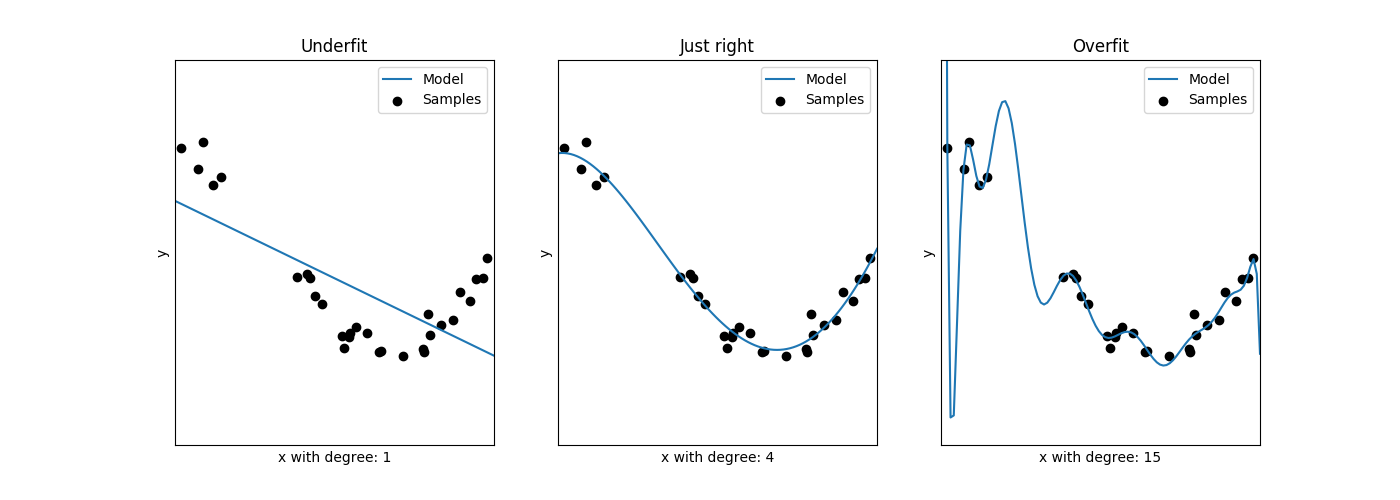
\includegraphics[width=\textwidth]{images/overfit_underfit.png}
\caption[Vergleich von Overfit zu Underfit]{Vergleich von Overfit zu Underfit}
\label{fig:under_overfit}
\end{figure}

Das Bias-Varianz-Dilemma ergibt sich durch die Komplexität eines Modells. Die Komplexität wird durch hinzufügen von Polynomen oder Features gesteigert.
Es ist daher sinnvoll die Modelle möglichst einfach zu gestalten oder einen Regularisierungsparameter zu verwenden.

\textbf{Ridge Regression}\\
Ridge Regression ist ein Linearer Regressions Algorithmus mit einem Regularisierungsparameter $\lambda$. Anhand diesem kann der Algorithmus die Koeffizienten der einzelnen Features verkleinern und somit die Komplexität reduzieren. Infolgedessen wird $\lambda$ auch Schrumpfparameter genannt. Je höher dieser gewählt wird, desto schwächer werden die Koeffizienten \cite{ridge, ridge_2}. Formel \eqref{eq:ridge} zeigt die Definition von Ridge Regression.

\begin{equation}
\label{eq:ridge}
J(\theta) = \frac{1}{2m} \sum_{i=1}^{N} (h_\theta(x^i) - y^i)^2 + \lambda \sum_{j=0}^{M} \theta_{j}^{2}
\end{equation}

Wichtig beim Ridge Algorithmus ist, dass die einzelnen Koeffizienten verkleinert werden, aber nie 0 erreichen. Das geeignetste Lambda hängt immer vom Datensatz ab und muss durch analysieren verschiedener Werte gefunden werden.

\textbf{Lasso Regression}\\
Ein weiterer Regularisierungs Algorithmus ist der Lasso Regression Algorithmus \eqref{eq:lasso}. Dieser fügt, wie der Ridge Regression auch, einen zusätzlichen $\lambda$ Parameter ein. Er nimmt dabei nicht das $\theta$ im Quadrat, sondern den absoluten Wert von $\theta$ und summiert diesen auf. Durch das kann der Algorithmus unwichtige Features auf 0 setzen und eliminieren. Wenn Features weggelassen werden, wird die Komplexität des Modells reduziert \cite{lasso}.

\begin{equation}\label{eq:lasso}
J(\theta) = \frac{1}{2m} \sum_{i=1}^{N} (h_\theta(x^i) - y^i)^2 + \lambda \sum_{j=0}^{M} |\theta_j|
\end{equation}

\subsubsection{$K$-Nearest Neighbour}
Der $K$-Nearest Neighbour Algorithmus (KNN) ist ein unsupervised Algorithmus und kann für Klassifizierungs- wie auch für Regressionsmodelle verwendet werden. In dieser Arbeit wird er als Regressionsmodell verwendet.\\
Der KNN-Algorithmus sucht für einen Datensatz die $K$ ähnlichsten Datensätze aus dem Trainingsset. Als Schätzung gibt er den Durchschnitt der gefundenen Werten ab \cite{knn_1}. KNN ist folgendermassen definiert \eqref{eq:knn_1}:

\begin{equation}\label{eq:knn_1}
\hat{y} = \frac{1}{K} \sum_{i=1}^{K} (y_{knj})
\end{equation}

Wobei $\hat{y}$ der geschätzte Wert darstellt, $K$ die Anzahl Datensätze, die für die Schätzung einbezogen werden und $y_{knj}$ die gefundenen beobachtungs Werte, die am nächsten zum gesuchten Punkt liegen.\\
Die Distanzberechnung von einem gesuchten Punkt kann mit unterschiedlichen Algorithmen berechnet werden. Häufig wird der Euklid, wie in Formel~\eqref{eq:euklid} gezeigt, verwendet, da er alle Dimensionen gleich behandelt. Wie beim quadratischen Fehlermodell, ist auch der Euklid anfällig auf grosse Ausreisser. Um das zu verhindern, kann der Manhatten oder Chebyshev Algorithmus verwendet werden. Beim Manhatten Algorithmus werden Querdistanzen höher gewichtet als gerade Distanzen. Im Gegensatz zum Chebyshev Algorithmus, bei dem alle Richtungen gleich gewichtet werden.

\begin{equation}\label{eq:euklid}
D(x, p_i) = \sqrt{(x - p_i)^2}
\end{equation}

Auch bei diesem Algorithmus trit die Gefahr von einem Underfit und Overfit auf. Wird $K$ zu gross gewählt, kommt es zu einem Underfit. Ist $K$ sehr klein kann es zu einem Overfit kommen. Das optimale $K$ hängt vom Datensatz und der gewünschten Performance ab. Abbildung \ref{fig:under_overfit_knn} zeigt den Vergleich von einem Underfit zu einem Overfit bei einem KNN Algorithmus.

\begin{figure}[ht]
\centering
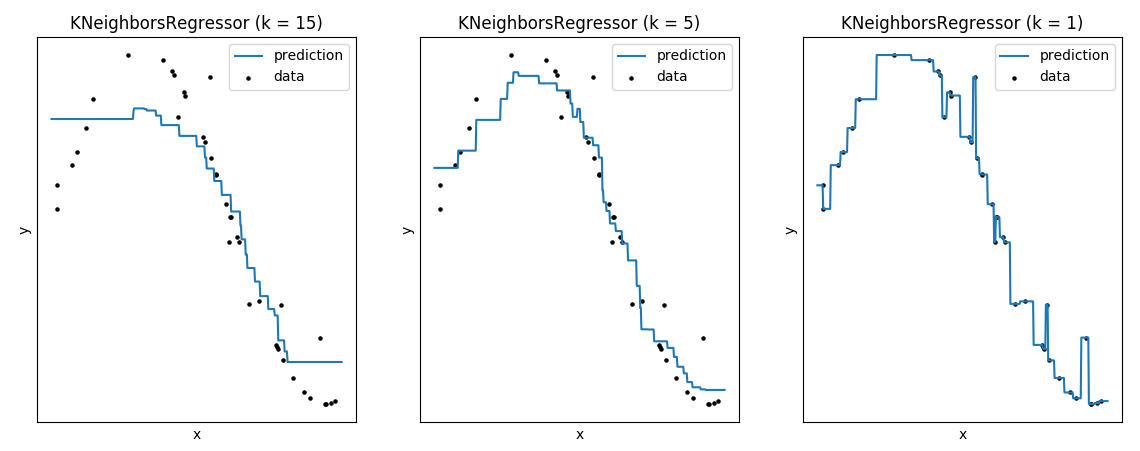
\includegraphics[width=\textwidth]{images/knears_overfit.png}
\caption[Vergleich von Overfit zu Underfit bei einem KNN]{Vergleich von Overfit zu Underfit bei einem KNN}
\label{fig:under_overfit_knn}
\end{figure}

Der KNN Algorithmus kann erweitert werden, indem näher gelegene Punkte stärker gewichtet werden als weiter entfernte. So ist der Algorithmus weniger anfällig auf unregelmässige Daten oder Ausreisser.\\
Für die Gewichtung eines Punktes wird folgende Formel verwendet~\eqref{eq:knn_weights}:

\begin{equation}
\label{eq:knn_weights}
W(x, p_i) = \frac{e^{(-D(x, p_i))}}{\sum_{i=1}^{K} e(-D(x, p_i))}
\end{equation}

$D(x, p_i)$ ist die Distanz vom gesuchten Punkt $x$ zum nächsten Punkt $i$ im Trainingsset. Da immer durch die Summe aller Distanzen dividiert wird, ist der Wert immer zwischen 0 und 1. Näher gelegene Punkte erhalten somit eine höhere Gewichtung $W$. Die Summe aller Gewichte ergibt immer 1.\\
Die Gewichtung wird mit dem gefundenen Beobachtungswert multipliziert, wie in Formel \eqref{eq:knn_with_weights} gezeigt. Die Durchschnittsberechnung muss nicht durchgeführt werden, da die Gewichtung normalisierte Werte zurückgibt \cite{knn_2, knn_3}.

\begin{equation}
\label{eq:knn_with_weights}
\hat{y} = \sum_{j=1}^{K} W(x_0, x_i) y_i
\end{equation}

\subsubsection{Tree Based Learning Algorithmen}
Ein anderer Ansatz von Machine Learning besteht aus den Tree Based Learning Algorithmen. Am verbreitetsten sind Classification and Regression Trees (CART), die von Breiman 1984 beschrieben wurden. Darunter existieren noch diverse ähnliche Algorithmen\footnote{ID3, C4.5, CHADI, MARS, Conditional Inference Trees}. Bei diesen Algorithmen handelt es sich grundsätzlich um supervised Algorithmen. Es existieren aber auch unsupervised Ansätze, die nicht Teil dieser Arbeit sind.

\textbf{Decision Trees}

\begin{figure}[h]\label{fig:decision_tree}
  \centering
  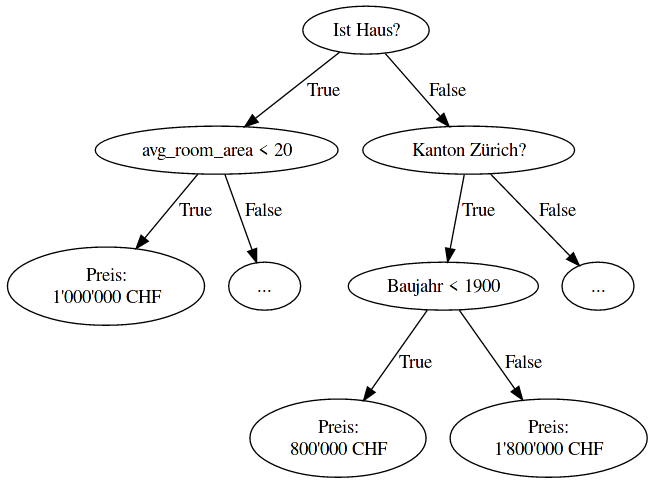
\includegraphics[width=0.7\textwidth]{images/decision_tree.png}
  \caption[Aufbau eines Decision Trees]{Aufbau eines Decision Trees}
\end{figure}

Ein Decision Tree (Entscheidungsbaum) ist eine Baumstruktur, die es erlaubt, Daten mithilfe von Entscheidungsregeln zu kategorisieren. Bei den Daten kann es sich sowohl um diskrete als auch um kontinuierliche Werte handeln.\\
Auf jedem Knoten des Entscheidungsbaumes wird ein Feature aus dem Datensatz ausgewählt und eine Teilung in seinem Wertebereich durchgeführt. Der Feature Raum wird somit in unterschiedliche, nicht überlappende Regionen aufgeteilt. Es gilt zu beachten, dass dasselbe Feature wiederholt als Entscheidungsregel verwendet werden kann.

Für eine Schätzung wird der Durchschnitt aller Werte in den Regionen $R_j$ berechnet, in die der zu schätzende Wert fällt.\\
Wie die  $J$ unterschiedliche Regionen aufgeteilt werden, hängt von der Kostenfunktion ab. Bei der Regression wird dafür den Residual Sum of Squares (RSS) verwendet. Das Ziel ist es die Regionen $R_1$, $R_2$ … $R_j$ so zu legen, dass der RSS minimiert wird. Das kann anhand der Formel \eqref{eq:decision_tree} erreicht werden.

\begin{equation}
\label{eq:decision_tree}
\sum_{j=1}^{J} \sum_{j \in R_j}^{} (y_i - \hat{y}_{R_j})^2
\end{equation}

Dabei ist $\hat{y}_{R_j}$ der durchschnittliche Beobachtungswert in der $j$-ten Region. Für eine Klassifikation werden andere Kostenfunktionen wie der Gini Coefficent oder Gini Impurity verwendet.

Da es aber mit steigender Anzahl von Datensätzen praktisch unmöglich wird, jede mögliche optimale Region durchzurechnen, wird ein “greedy” Ansatz verwendet. Greedy deshalb, weil die nächstbeste Teilung nur mit den aktuell vorhandenen Regionen berechnet wird. Es wird nicht rekursiv vorausberechnet um mit weiteren Teilungen ein theoretisch besseren Baum zu erstellen. So wird nur ein lokales und kein globales Optimum gefunden. Die Aufteilung einer Region in zwei unterschiedliche Regionen nennt sich “recursive binary splitting” und wird in Formel \eqref{eq:splitting} gezeigt. Dabei gilt die Bedingung für die zuteilende Region $R$, wobei $s$ die Entscheidungsregel ist.

\begin{equation}\label{eq:splitting}
R_1(j,s) = \{X|X_j < s\} \text{ and } R_2(j,s) = \{X|X_j \geq s\}
\end{equation}

Diese Splits werden solange rekursiv ausgeführt, bis eine der folgenden Abbruchbedingungen erfüllt ist:

\begin{itemize}
\item Die minimale Anzahl an Datensätzen in einer Region ist erreicht.
\item Die maximale Tiefe wurde für einen Teilbaum erreicht.
\item Ein erneuter Split bringt keine besseren Ergebnisse.
\end{itemize}

Die Vorteile vom Decision Tree bestehen darin, dass der generierte Baum einfach verständlich und lesbar ist, da das Endresultat ein geordneter und gerichteter Baum ist. Dadurch lässt sich dieser bei Bedarf auch gut visualisieren und Predictions können manuell überprüft werden, sofern der Baum nicht zu gross ist.\\
Decision Trees neigen jedoch gerne zu Overfitting. Dagegen hilft einerseits Pruning, andererseits Ensemblemethoden.\\
Pruning eliminiert bestehende Knoten, die sich als irrelevant herausstellen, anhand einem Regularisierungsparameter $\lambda$. Dieses Parameter ist ähnlich wie beim Lasso Algorithmus. Pruning ist jedoch nicht so verbreitet wie die Ensamblemethoden.

\textbf{Random Forest}\\
Der Random Forest gehört in die Kategorie der Ensemblemethoden. Es handelt sich hierbei um einen erweiterten Bootstrap Aggregating (Bagging) Algorithmus und wurde von Breiman entwickelt. Bagging reduziert die Varianz indem der Algorithmus mehrere Bäume aus dem Datensatz generiert und diese einzeln trainiert.  Die Bäume trainieren jeweils aus einer zufälligen Teilmenge des ganzen Datensatzes. Für die Schätzung wird der Durchschnitt aller Bäume $B$ verwendet, wie in Formel \eqref{eq:random_forest} gezeigt. Dabei ist $f^{(b)}$ die Schätzung für den b-ten Baum.

\begin{equation}
\label{eq:random_forest}
\hat{f_{bag}} = \frac{1}{B} \sum_{b=1}^{B} f^{(b)} (X)
\end{equation}

Es kann auftreten, dass die Bäume untereinander korrelieren und sich so die Vorhersage verschlechtert. Der Random Forest Algorithmus eliminiert dieses Problem, indem er bei jeder Teilung in einem Subset nicht alle, sondern nur weniger, zufällig ausgewählte Features verwendet. Die Bäume sollten möglichst gross werden und es sollte kein Pruning durchgeführt werden.\\
Breiman hat in einem Theorem bewiesen, dass mit dieser Methode kein Overfitting stattfinden kann, sofern genügend Trees verwendet werden \cite{random_forest, random_forest_1}.
%
\newpage
\textbf{Extra Trees}\\
Extra Trees (Extremely Randomized Trees) ist eine abgeleitete Variante des Random Forests. Im Unterschied zu Random Forests bezieht Extra Trees immer alle Datensätze in die Berechnungen der Decision Trees ein. Dadurch wird der Bias besser minimiert als wenn nur ein Teildatensatz verwendet wird. Zudem werden die Splits in den Knoten komplett zufällig gewählt um die Varianz besser reduzieren zu können. In der Studie wurde empirisch bewiesen, dass der Extra Trees Algorithmus im allgemeinen besser performed als vergleichbare Ensemble Algorithmen \cite{extrem_forest}.

\textbf{XGBoost}\\
XGBoost steht für Extreme Gradient Boosting und gehört ebenfalls zur Familie der Ensemble-Algorithmen \cite{xgboost}.\\
Im Unterschied zu Random Forest oder Extra Trees bauen die trainierten Decision Trees aufeinander auf und lernen von den Fehlern der vorher trainierten Decision Trees. Dies wird solange wiederholt, bis der Fehler so klein ist, dass keine Verbesserung mehr erreicht werden kann. Dieses Vorgehen wird Boosting genannt und gehört zur Kategorie des additiven Lernens. Im Allgemeinen sieht die Formel für Gradient Boosting folgendermassen aus \eqref{eq:xgboost}:

\begin{flalign}
\label{eq:xgboost}
\begin{split}
\hat{y}_{i}^{(0)} &= 0\\
\hat{y}_{i}^{(1)} &= f_1(x_i) = \hat{y}_{i}^{(0)} + f_1(x_i)\\
\hat{y}_{i}^{(2)} &= f_1(x_i) + f_2(x_i)= \hat{y}_{i}^{(1)} + f_2(x_i)\\
\text{\ldots}\\
\hat{y}_{i}^{(t)} &= \sum_{k=1}^{t} f_k(x_i) = \hat{y}_{i}^{(t-1)} + f_t(x_i)
\end{split}
\end{flalign}

$\hat{y}_{i}^{(t)}$ ist dabei der zu schätzende Wert für Datensatz i vom Decision Tree t. $f_t$ ist die Funktion vom Decision Tree t.

Die Zielfunktion, in Formel \eqref{eq:xgboost_target} dargestellt, für XGBoost funktioniert im Endeffekt ähnlich wie bei einer Lasso Regression, indem der Residual Sum of Squares (RSS) berechnet wird (hier $l()$).
Um ein Overfitting zu verhindern, wird die Regularisierungsfunktion $\Omega(f)$ hinzugenommen. Dieser Wert berechnet die Komplexität des Modells und hält die Parameter für den Decision Tree klein \cite{xgboost_1, xgboost_2}.

\begin{equation}
\label{eq:xgboost_target}
obj^{(t)} = \sum_{i=1}^{n} l(y_i, \hat{y}_{i}^{(t)}) + \sum_{i=1}^{t} \Omega(f_i)
\end{equation}

Kritik an diesem und verwandten Algorithmen wird in \cite{critic} geäussert. Darin wird beschrieben, dass für Daten mit inkorrekten Einträgen die Boost Algorithmen versuchen, diese Unreinheiten zu stark zu kompensieren. Dadurch erhalten sie so eine schlechtere Performance. Das kann aber mit Feature Engineering minimiert werden.
%
\subsubsection{Isolation Forest}
Der Isolation Forest Algorithmus ist ein neuerer Outlier Detection Algorithmus\footnote{Algorithmus zur Erkennung von Ausreissern.}. Der Algorithmus wurde im Jahr 2008 von Fei Tony Liu, Kai Ming Ting und Zhi-Hua Zhou entwickelt und vorgestellt. Outlier Detection ist ein wichtiger Teil beim Machine Learning Prozess. Mit diesem werden Datensätze herausgefiltert, die zu stark von den erwarteten Grössen abweichen und somit einen Ausreisser darstellen \cite{isolation_forest_1}.\\
Bekannte Outlier Detection Algorithmen versuchen mit Hilfe der Distanz oder der Dichte die Ausreisser zu erkennen. Der One-Class SVM sowie der Local Outlier Factor (LOF) messen die Dichte, wobei K-Nearest Neighbour die Distanz berechnet \cite{isolation_forest_2}.\\
Diese erzielen bei unregelmässig verteilten Ausreisser ein gutes Ergebnis. Sind die Ausreisser aber als Gruppe vorhanden, haben Distanz- oder Dichtebasierte Algorithmen mehr Mühe diese als Ausreisser zu erkennen \cite{isolation_forest_3}.

Der Isolation Forest geht hier einen anderen Weg. Er geht davon aus, dass sich Ausreisser besser isolieren lassen als normale Datensätze.\\
Unter Isolieren ist das Separieren eines Beobachtungswerts von den restlichen Werten gemeint. Dafür wird der Datensatz kontinuierlich partitioniert, bis er alleine in einer Partition vorkommt oder die maximale Anzahl an Partitionen erreicht wurde. Die Aufteilung der Partitionen wird als Binary Tree dargestellt. Jeder Knoten repräsentiert eine Eingrenzung und hat, wenn er kein Blatt ist, zwei Kinderknoten. Die Grenzen werden wie bei Extra Trees zufällig ausgewählt.

\begin{figure}[h]
  \centering
  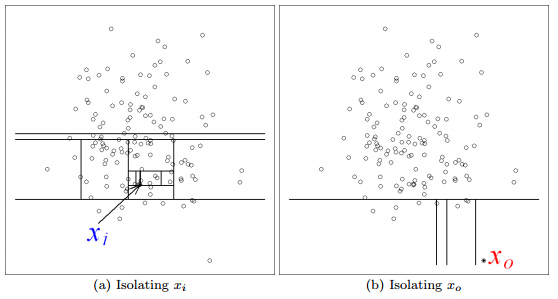
\includegraphics[width=0.8\textwidth]{images/isolation_forest.png}
  \caption[Isolation Forest]{Isolation Forest}%
  \label{fig:hintergrund_isolation_forest}
\end{figure}

Die Pfadlänge wird durch die Anzahl Knoten, die vom Root Node bis zum Ende durchlaufen werden müssen, bestimmt. Da die Partitionsgrenzen zufällig gewählt werden, führt man diese Isolation mehrmals für einen Punkt durch und nimmt davon die durchschnittliche Länge. Je kürzer ein Pfad ist, desto eher handelt es sich um einen Ausreisser. Denn dieser konnte schneller isoliert werden. Abbildung \ref{fig:hintergrund_isolation_forest} zeigt die Isolation  eines normalen Beobachtungswert $Xi$, wobei $b$ die Isolation eines Ausreisser $X_0$ darstellt.

% Newpage if not on new page TODO
Der Anomaly Score wird mit Hilfe der nicht erfolgreichen Suche eines Binary Search Tree berechnet. Dabei ist n die Anzahl Knoten, $E(h(x))$ die durchschnittliche Pfadlänge und $c(n)$ die durchschnittliche Kostenfunktion einer nicht erfolgreichen Suche im Binary Search Tree. Die Formel dafür sieht wie folgt aus:

\begin{equation}\label{eq:isolation}
s(x, n) = 2^{-\frac{E(h(x))}{c(n)}}
\end{equation}

Die Funktion $s(x, n)$ gibt immer einen Wert zwischen 0 und 1 zurück. Wobei 1 einem klarem Ausreisser entspricht \cite{isolation_forest_2}.
\newpage
\clearpage
% NUR ZIEL SYSTEM (Das was wir entwickeln) WIE wird mit situationen gearbeitet, was wir machen
\section{Architektur}
Im folgenden Kapitel wird schematisch der gesamte Aufbau der Komponenten erklärt. Es handelt sich hierbei um ein Python Projekt das drei Module besitzt. Die Module sind nach ihren Hauptaufgaben aufgeteilt. Da es sich nicht um eine klassische Applikation handelt, werden die einzelnen Komponenten erläutert.
%
\subsection{Systemaufbau}
Abbildung \ref{fig:system} zeigt den ganzen Systemaufbau dieser Arbeit, wobei der blaue Bereich die Komponenten beinhaltet, die auf unserer Infrastruktur betrieben sind. Das ganze wird auf einem Linux Server gehosted.\\
\begin{figure}[ht]
\centering
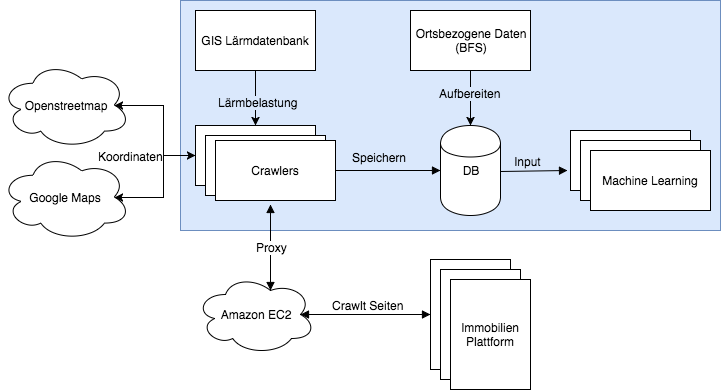
\includegraphics[width=\textwidth]{images/Architektur.png}
\caption[Systemaufbau des Projektes]{Systemaufbau des Projektes}%
\label{fig:system}
\end{figure}
Es gibt diverse Schnittstellen zu externen APIs oder Datenbanken, die wir verwenden um zusätzliche Informationen zu bekommen. Die drei wichtigsten Komponenten sind:
\begin{description}
\item[Crawler:] Sie sammeln die Immobiliendaten auf den verschiedenen Portalen. Die Crawler besitzen diverse Schnittstellen zu anderen Anbieter wie auch Datenbanken. 
\item[Datenbank:] Die Datenbank ist die zentrale Speicherstelle für unsere Inserate. Die Datenbank wurde ganz am Anfang mit ortsbezogenen Daten vom Bundesamt für Statistik befüllt. 
\item[Machine Learning:] Die Daten für das Datenset werden aus der Datenbank geladen und für die verschiedenen Algorithmen bereitgestellt.
\end{description}
In den folgenden Kapiteln wird auf diese drei Komponente genauer eingegangen.
%
\subsection{Aufbau Crawler}
Für diese Arbeit wird Scrapy als Webcrawler verwendet. Scrapy ist ein mächtiges, in Python geschriebenes, Open Source Crawler Framework.\\
Scrapy wurde ausgewählt, da es sich als Python Framework sehr gut in die Entwicklungsumgebung einfügt und es einfach anzuwenden ist \cite{scrapy}.\\
Weiter bietet Scrapy eine Item Pipeline an, um gesammelte Daten weiter zu verarbeiten. Der Vorteil der Pipeline ist, dass es erlaubt unabhängige sowie auch abhängige Schritte der Reihe nach isoliert durchzuführen. Abbildung \ref{fig:scrapy} zeigt den Aufbau der verwendeten Pipeline für das Sammeln von Immobiliendaten.\\[2ex]
\begin{figure}[h!]
\centering

\includegraphics[width=\textwidth]{images/scrapy.png}
\caption[Scrapy Pipeline]{Scrapy Pipeline}%
\label{fig:scrapy}
\end{figure}
\newline
%
\textbf{Crawlen der Webseiten}\\
Für das Crawlen der Kaufobjekte auf einer Immobilienplattform werden fokussierte Crawler verwendet. Da es zahlreiche Immobilienplattformen in der Schweiz gibt, wurden vier der grössten Plattformen ausgesucht, siehe Tabelle \ref{tab:portals}. Die Grösse definiert sich an der Anzahl Inseraten, die auf einer Seite ausgeschrieben sind. Dafür wurde die Rankingliste von Comparis genommen.\\
Um nicht als Crawler aufzufallen wurde mit Scrapoxy auf Amazon mehrere Proxy Instanzen gestartet. Diese wurden im 10-Minuten Takt terminiert und neue gestartet, um immer frische IP-Adressen zu erhalten. Da Amazon keine schweizer Server anbietet, konnten nur Portale angesteuert werden, die ausländische IP-Adressen zulassen. Comparis als grösstes Portal sperrt alle ausländischen IP-Adressen und ist so für uns nicht benutzbar.\\[2ex]
\begin{table*}[ht]
\centering
\ra{1.3}
\begin{tabular}{@{}lr@{}}
\toprule
Portal & Anzahl Inserate \\
\midrule
Homegate & 85'358\\
Immoscout & 65'543\\
Newhome & 42'804\\
Urbanhome & 27'092\\
\bottomrule
\end{tabular}
\caption{Anzahl verfügbare Inserate}
\label{tab:portals}
\end{table*}
%
Für jedes Immobilienportal erstellten wir einen eigenen Crawler. Um alle Immobilien der Schweiz zu erhalten, haben die Crawler 26 Einstiegs URLs. Jede URL deckt einen Kanton ab. Der Grund dafür ist, dass keine Immobilienplattform eine gesamtschweizerische Übersicht über ihre Immobilien anbietet. Die grösste Übersicht deckt einen ganzen Kanton ab. Punktuell mussten die URLs noch weiter verfeinert werden, da die Anzahl Resultate begrenzt waren.\\
Diese Einstiegsseiten beinhalten eine Liste aller verfügbaren Immobilien in diesem Kanton. Um an die detaillierten Informationen zu kommen, muss der Link zum Inserat extrahiert werden und in einem zweiten Schritt aufgerufen werden.
Demzufolge braucht ein Crawler fürs Portal zwei verschiedene Parser. Einer der die Übersicht und einer der die Detailseite parsed.\\[2ex]
%
Das Parsen der Seite erfolgt mit Hilfe von XPath. Die XPath Regeln wurden für alle Seiten im Voraus definiert. Bis auf die Bilder werden alle Informationen, die der Verkäufer eingeben kann, gesammelt (siehe Anhang).\\
Viele Immobilien sind nur wenige Tage online. Um später die Möglichkeit zu haben, weitere Informationen aus den Inseraten zu beschaffen, wurde zusätzlich der ganze HTML Code zum Inserat gespeichert.\\[2ex] 
%
\textbf{Zuordnung Gemeinde}\\
Vom Bundesamt für Statistik werden geobasierte Informationen der Gemeinden und Kantonen bezogen. Deshalb muss das Inserat anhand seiner Adresse einer Gemeinde zugeordnet werden. Dies geschieht in einem mehrstufigen Prozess.\\
Als erstes wird die Postleitzahl und die Ortschaft vom Inserat extrahiert. Danach wird anhand der Postleitzahl in der Datenbank den Gemeindenamen gesucht. Stimmt dieser mit dem gecrawlten Namen überein, kann die Zuordnung erfolgen.\\
Stimmt der Gemeindename nicht überein, existiert zusätzlich eine Zusatzspalte mit Alternativnamen für die Gemeinde.  Dies sind meist ältere Namen von Gemeinden die durch eine Fusion nicht mehr existieren.\\
Wird der gecrawlte Namen auch nicht in den Alternativnamen gefunden, kann keine Zuordnung durchgeführt werden.\\[2ex]
%
\textbf{Dublettencheck}\\
Es ist möglich, dass ein Inserat bei mehreren Plattformen online gestellt wird. Da es nicht optimal ist, wenn ein Inserat zweimal in unserem Datensatz vorkommt, wird versucht möglichst früh Dubletten zu erkennen und herauszufiltern. Der Dublettencheck überprüft die Übereinstimmung von Ortschaft, Objekttyp, Preis, Wohnfläche und Anzahl Zimmer. Sind diese Eigenschaften gleich, wird das Inserat ignoriert.\\[2ex]
%
\textbf{Auslesen der Tags}\\
Die Beschreibung eines Inserates, wie auch die Charakteristik, beinhaltet viele Informationen. Zum einen werden die Eckdaten nochmals in prosa formuliert. Zum Anderen wird die Innen- und Ausseneinrichtung, sowie die Umgebung beschrieben. Hier bietet sich an, diesen Text anhand von Natural Language Processing zu untersuchen. Dazu werden die wichtigsten Wörter extrahiert und als JSON-Liste abgespeichert.\\
Das NLTK-Module, das für solche Aufgaben gedacht ist, hat aber nur sehr wenige Stop-Wörter. Somit mussten wir uns eine eigene Stoppwörterliste zusammenstellen. Auch für die Übersetzung der einzelnen Ausdrücke haben wir ein eigenes Dictionary verwendet.\\[2ex]
%
\textbf{Koordinaten setzen}\\
Um die Koordinaten zu setzen, braucht es eine Strassenanschrift. Ist diese nicht vorhanden werden auch keine Koordinaten gesetzt. Das Beschaffen der Koordinaten ist ein mehrstufiger Prozess. Da von Google Maps eine Limite von 2500 Requests pro Tag existiert, wird versucht zuerst über die Openstreetmap API die Koordinaten zu beschaffen. Openstreetmap hat vergleichsweise zu Google viel weniger Einträge. Wenn bei Openstreetmap keine Koordinaten gefunden werden, wird die Google Maps API angesteuert.\\[2ex]
%
\textbf{Lärmbelastung}\\
Dieser Schritt ist der einzige in der Pipeline, der abhängig vom vorherigen Schritt ist. Denn sind keine Koordinaten vorhanden, kann auch keine Lärmbelastung berechnet werden. Die Lärmbelastung für die ganze Schweiz liegt in einem vom Bundesamt für Umwelt bereitgestellten GDAL-Format vor. Hierfür werden die Koordinaten in das Schweizer Koordinatensystem LV03 umgerechnet. Mit diesen kann in einem nächsten Schritt die Lärmbelastung berechnet werden.\\[2ex]
%
\textbf{Speichern}\\
Schlussendlich wird das gecrawlte und ergänzte Item in die Datenbank gespeichert.
%
%
\subsection{Datenbank}
Für die Datenbank wurde PostgreSQL\footnote{https://www.postgresql.org/} eingesetzt. Die Datenbank besteht aus drei Tabellen. In der Haupttabelle \textit{advertisements} sind alle Inserate der verschiedenen Immobilienportale gespeichert. In der Tabelle \textit{municipalities} sind alle ortsbezogenen Daten zu den Gemeinden und Kantonen abgelegt. Die Daten stammen vom Bundesamt für Statistik\footnote{https://www.bfs.admin.ch/bfs/de/home/statistiken/querschnittsthemen/raeumliche-analysen/raeumliche-gliederungen.assetdetail.2118475.html}. Für die Auswertung reichen die verschiedenen IDs der kategorischen Bezeichnungen. Für die Auswertung wurde stichpunktartig ein Mapping erstellt.
Die dritte Tabelle \textit{object\_types} beinhaltet alle Objekttypen, die beim Sammeln gefunden wurden. Sie wird autonom von den Crawlern befüllt.
\begin{figure}[h!]
\centering
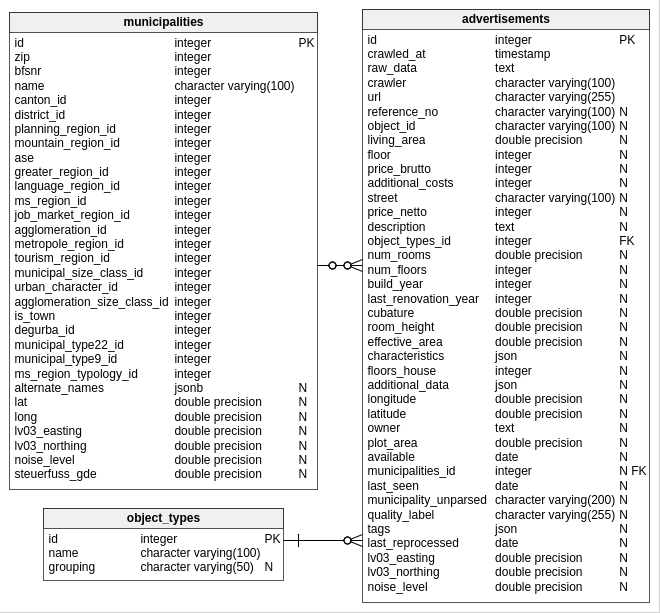
\includegraphics[width=0.9\textwidth]{images/erm.png}
\caption[Datenbankschema]{Datenbankschema}%
\label{fig:db}
\end{figure}
\newline
%
\subsection{Machine Learning}
Für Machine Learning wurde hauptsächlich mit Scikit-Learn gearbeitet \cite{scikit}. Scikit-Learn ist eine in Python geschriebene Machine Learning Library mit einer grossen Community. Punktuell wurden noch weitere ML Algorithmen verwendet, die nicht in Scikit-Learn vorhanden sind, dies wird jeweils separat erwähnt.\\[2ex]
%
Bei jedem Durchgang werden die Daten von der Datenbank geladen und denormalisiert. Da das Laden der Daten von der Datenbank Zeitintensiv ist, werden die Daten lokal zwischengespeichert.\\
Anschliessend wird ein Feature Engineering durchgeführt, bei dem diverse Daten transformiert, ergänzt oder gelöscht werden. Als weiteren Schritt, wird die Outlier Detection durchgeführt und am Ende werden diverse Machine Learning Algorithmen durchgetestet.\\[2ex]
%
\begin{figure}[h!]
\centering
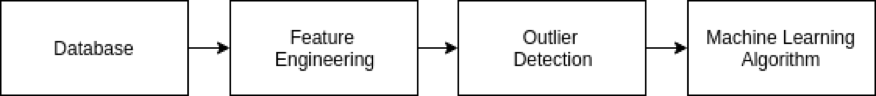
\includegraphics[width=0.9\textwidth]{images/machine_learning_pipeline.png}
\caption[Pipeline für Machine Learning]{Pipeline für Machine Learning}%
\label{fig:ml_pipeline}
\end{figure}
\newline
%
Um den ganzen Prozess einfacher zu handhaben, wurden alle Transformationen und Aktionen in möglichst kleine Funktionen verpackt, die in einer Pipeline kombiniert werden können. Somit können nach Wunsch einzelne Funktionen deaktiviert werden. Die Piepeline wird anhand einer JSON-Liste definiert. Diese Liste wird vom Programm eingelesen und der reihe nach abgearbeitet.\\[2ex]
%
Für jeden der Algorithmen wurden die diversen Parameter mit der GridSearchCV Komponente von scikit-learn durchgetestet. GridSearchCV testet für jeden Algorithmus alle Parameter mit einer Crossvalidation und gibt am Ende die Parameterwerte mit dem besten Resultat zurück. Bottleneck ist dabei die benötigte Zeit. Je nachdem wie viele Kombinationen durchgeführt werden müssen, kann das über einen Tag dauern.\\
Um nicht jedesmal eine Crossvalidation durchzuführen, werden die besten Resultate in eine Konfigurationsdatei geschrieben.\\
Der Einzige Algorithmus der nicht vom Scikit-Learn stammt, ist der XGBoost Algirthmus. Dieser wurde von Github heruntergeladen, kompiliert und das Python Paket installiert.
%
%
\subsection{Code Struktur}
Der gesamte Code mit Dokumentation wird ein einem Git Repositroy auf Github verwaltet. Git ist ein Versionsverwaltungstool. Es zeichnet auf, wer wann welche Änderungen an welchen Daten gemacht hat.\\
Die grobe Ordnerstruktur des Projektes sieht wie folgt aus:
\begin{verbatim}
immo/
  crawler
    crawler
      pipelines        # Definitionen der Pipelines
      spiders          # Definitionen der spiders
      ...
    ...
  models               # Objektdefinition
  scikit               # Machine Leraning 
    main.py            # Hauptdatei zum Starten der Pipeline
    pipeline.py        # Definitionen der verschiedenen ML-Algorithmen
    helper.py          # Anzeigen der Resultatstatistik
    data_analysis.py   # Holen und analysieren der Daten
    settings.json      # Speicherung der besten Parameter
    ...
  commands.json        # Definition der Pipeline
  ...
report                 # \LaTeX Report
daten                  # Import Daten für Datenbank
\end{verbatim}

\newpage
%
\clearpage
\section{Validierung}
Um die Forschungsfragen zu beantworten, haben wir die gesammelten Immobiliendaten auf Verwertbarkeit analysiert und gefiltert.\\
Bei den Machine Learning Algorithmen haben wir den MAPE sowie der MdAPE als wichtiges Performanzkriterium genommen. Weiter war uns wichtig, wie viele Inserate können mit einer Abweichung von 10\% geschätzt werden.\\
Gewisse Daten haben so extreme Werte, dass sie die Diagramme verzerren und so eine Aussage über die Daten erschweren. Deshalb werden diese Werte für die Validation ignoriert. Dabei handelt es sich um insgesamt 751 Inserate. Weiter wurden 12’219 Inserate weggelassen, da bei diesen der Kaufpreis fehlte.
Im nächsten Kapitel wird der Iterative Vorgang beschrieben.
%
\subsection{Gesammelte Daten}
Insgesamt konnten 162’225 Immobilieninserate in einem Zeitraum von 5 Monaten gesammelt werden. Davon stammen die meisten vom Immoscout24 Portal, was in Tabelle \ref{tab:crawled_data} ersichtlich ist.
\begin{table*}[ht]
\centering
\ra{1.3}
\begin{tabular}{@{}lrr@{}}
\toprule
Portal & Anzahl gesammelte Inserate & Anzahl verwendete Inserate \\
\midrule
Immoscout & 94'611 & 46'226\\
Homegate & 34'115 & 19'568\\
Newhome & 32'600 & 19'011\\
Urbanhome & 2'047 & 1'040\\
\bottomrule
\end{tabular}
\caption{Auswertung der gesmmelten Daten}
\label{tab:crawled_data}
\end{table*}
%
Von den insgesamt 162’225 Inseraten wurden 77’608 ungültige Inserate herausgefiltert. 
Dabei handelte es sich mehrheitlich um fehlerhafte Inserate oder Inserate, bei denen wichtige Kennwerte fehlten.\\
Insgesamt konnten 83’107 Wohungen und 65’430 Häuser gesammelt werden. Die restlichen Inserate waren Lagerräume oder nicht definierte Immobilientypen.\\
Weiter konnte für 83\% aller Inserate, mit einer vollständigen Adresse eine Lärmbelastung berechnet werden. Ebenso konnten für 99\% aller Inserate eine Gemeinde zugeordnet werden.\\
Die meisten Inserate haben eine Angabe über die Anzahl Zimmer und Wohnfläche. Gefolgt vom Baujahr und der Anzahl an Stockwerken, falls es mehrere besitzt. Die Raumhöhe oder die Kubatur wird dagegen nur selten angegeben. So auch die effektive Fläche einer Immobilie. Abbildung \ref{fig:features} zeigt den prozentualen Anteil der fehlenden Kennwerte.\\[2ex]
\begin{figure}[h!]
\centering
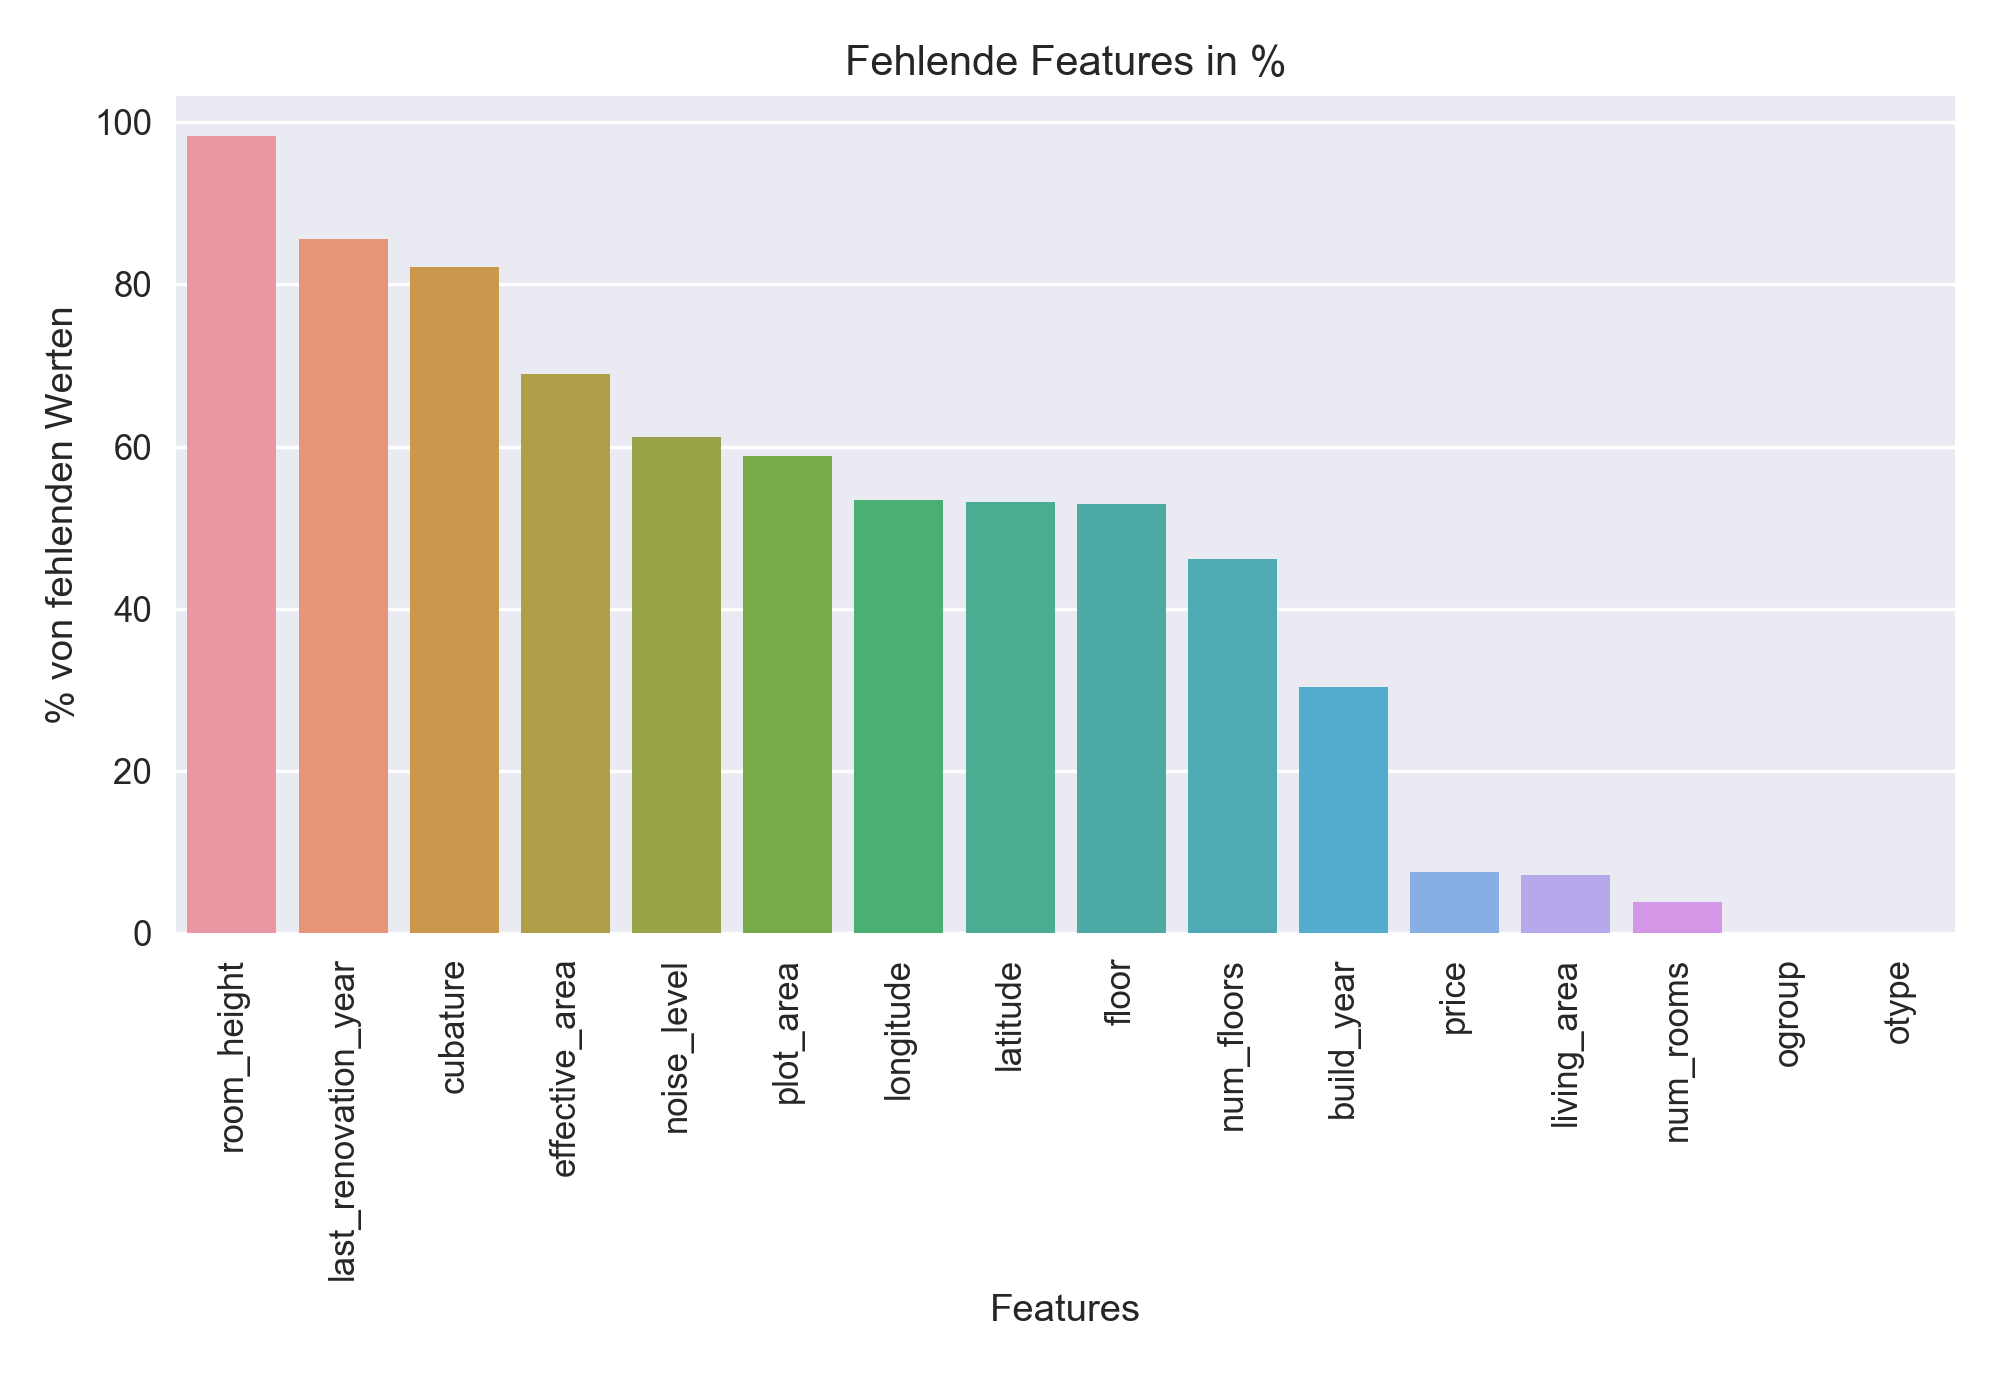
\includegraphics[width=0.9\textwidth]{images/missing_values.png}
\caption[Anzahl der vorkommenden Features]{Anzahl der vorkommenden Features}%
\label{fig:features}
\end{figure}
\newline
%
Die Crawler wurden nie über eine längere Zeit gesperrt. Vereinzelt kam es zu Blockierungen, die jedoch, durch das Starten neuer Proxyinstanzen, umgehen werden konnten. Der Zeitaufwand um ein Portal bei fünf gleichzeitigen Verbindungen und einer Download Delay von zwei Sekunden zu crawlen, lag im Schnitt bei 4 Stunden. Dementsprechend wurden in dieser Zeit etwa 100 Proxyinstanzen gestartet.\\[2ex]
%
Die Datenqualität ist eher mässig, da viele Inserate erst gar nicht für ein Trainingsdatensatz verwendet werden können. Um dem entgegenzuwirken, wurde versucht durch Feature Engineering fehlende Daten zu berechnen.
%
\subsubsection{Kaufpreis}
Abbildung \ref{fig:price} zeigt die Verteilung des Kaufpreises. Dabei sieht man, dass dieser nicht normalverteilt ist (\ref{fig:price_normal}). Es besteht eine positive Skenwess, was für eine Lineare Regression nicht optimal ist. Wird der Log-Wert des Preises genommen (\ref{fig:price_log}), kann eine Annäherung an eine Normalverteilung erreicht werden. Dies gilt es zu beachten, wenn später mit einer Linearen Regression gearbeitet wird.
Tabelle () zeigt die beschreibenden statistischen Werte des Preises.
%
\begin{figure}[ht]
\begin{subfigure}{.5\textwidth}
  \centering
  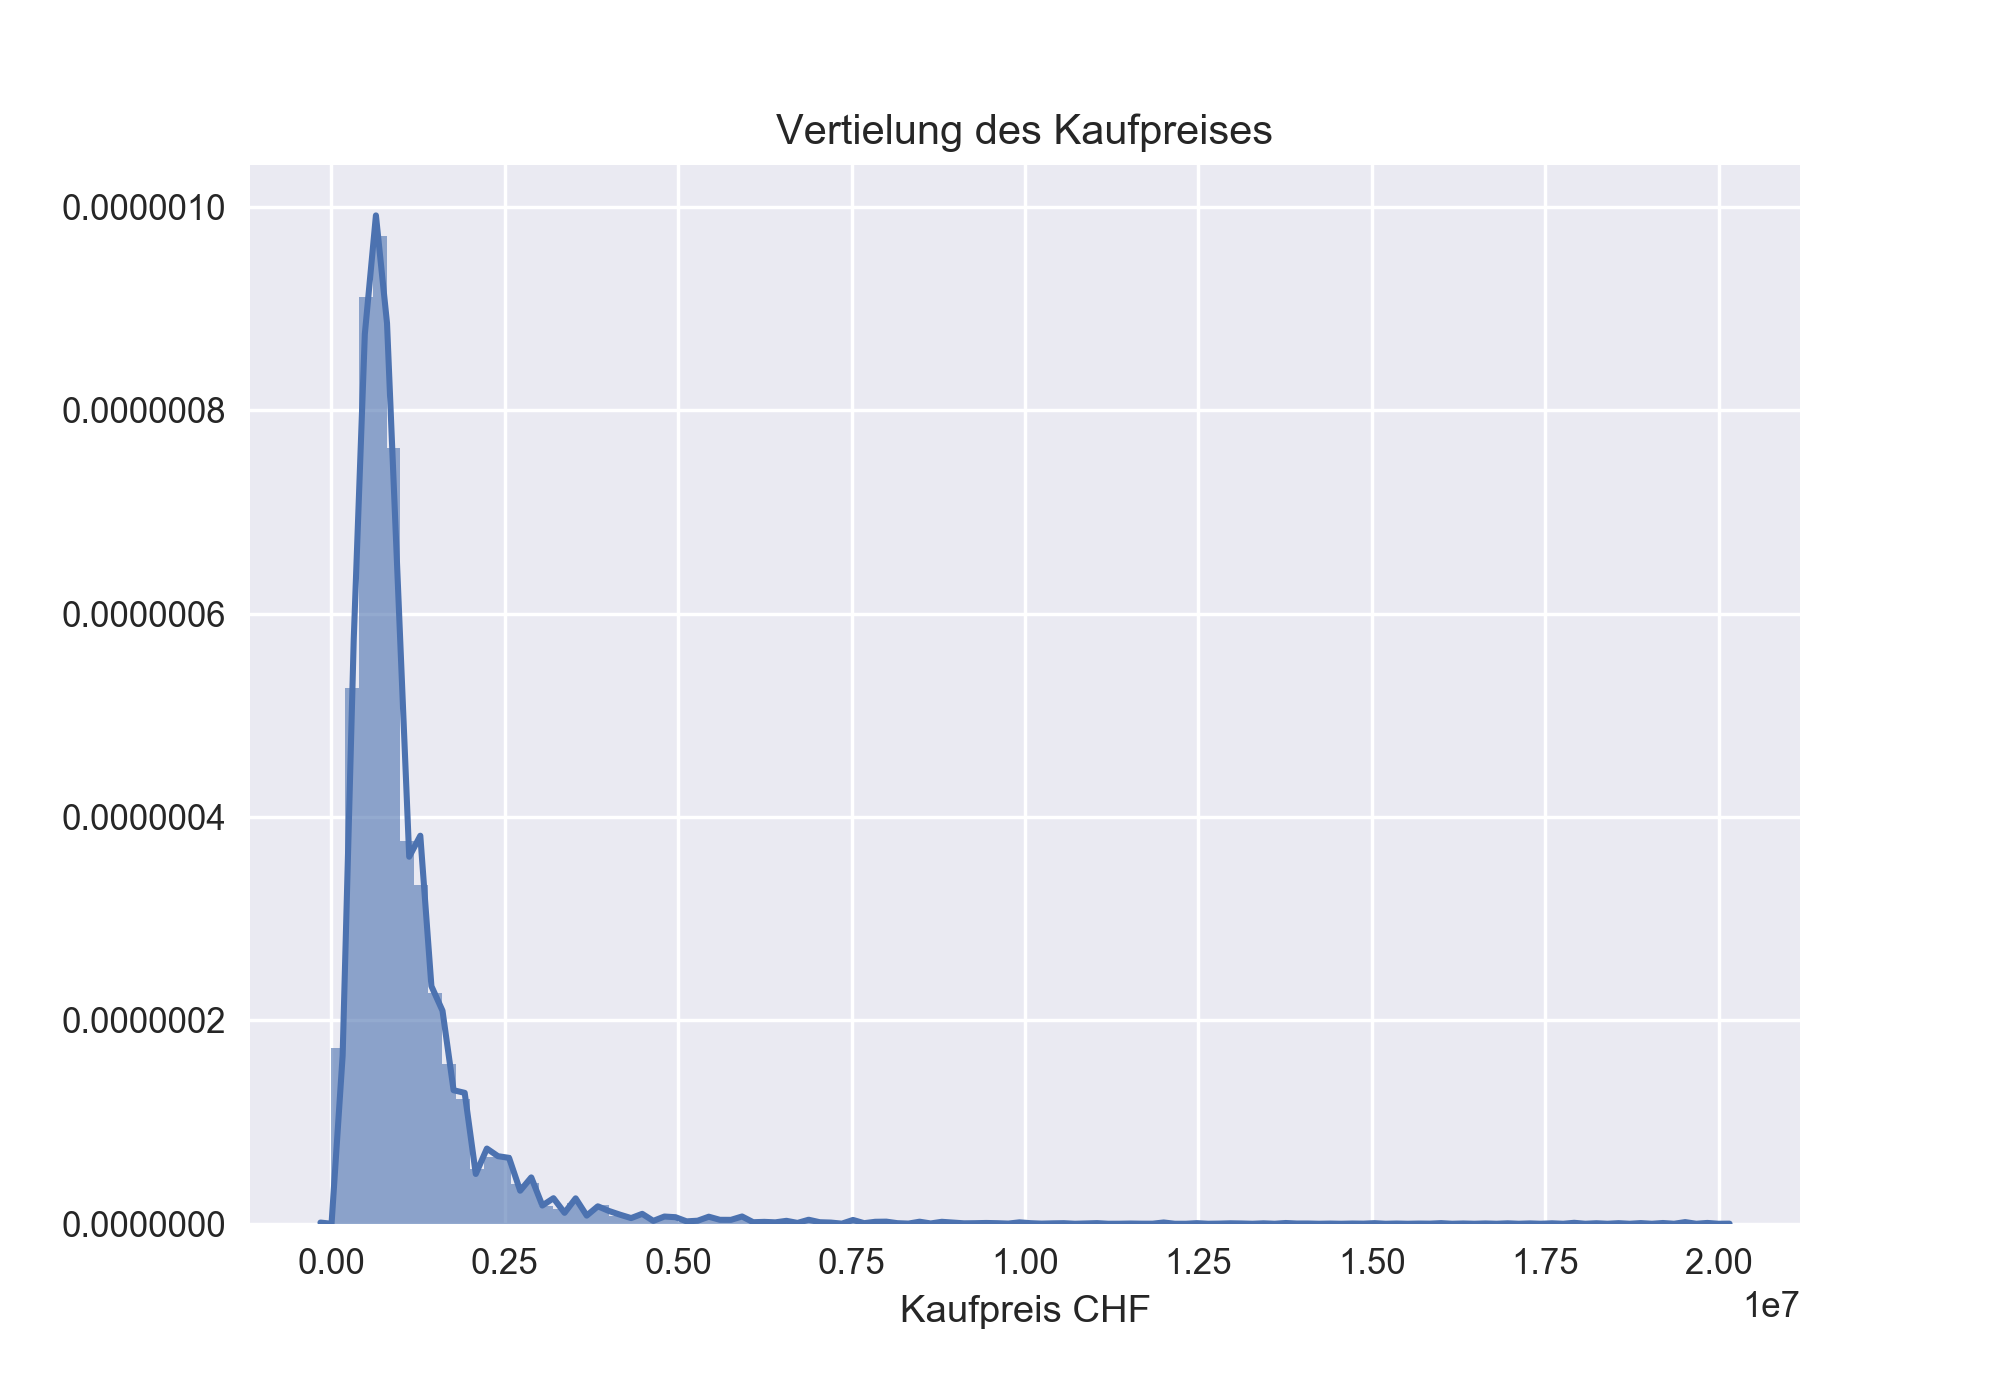
\includegraphics[width=\linewidth]{images/Verteilung_des_kauf_preises.png}
  \caption[Verteilung des Kaufpreises aller Immobilien]{Verteilung des Kaufpreises aller Immobilien}
  \label{fig:price_normal}
\end{subfigure}%
\begin{subfigure}{.5\textwidth}
  \centering
  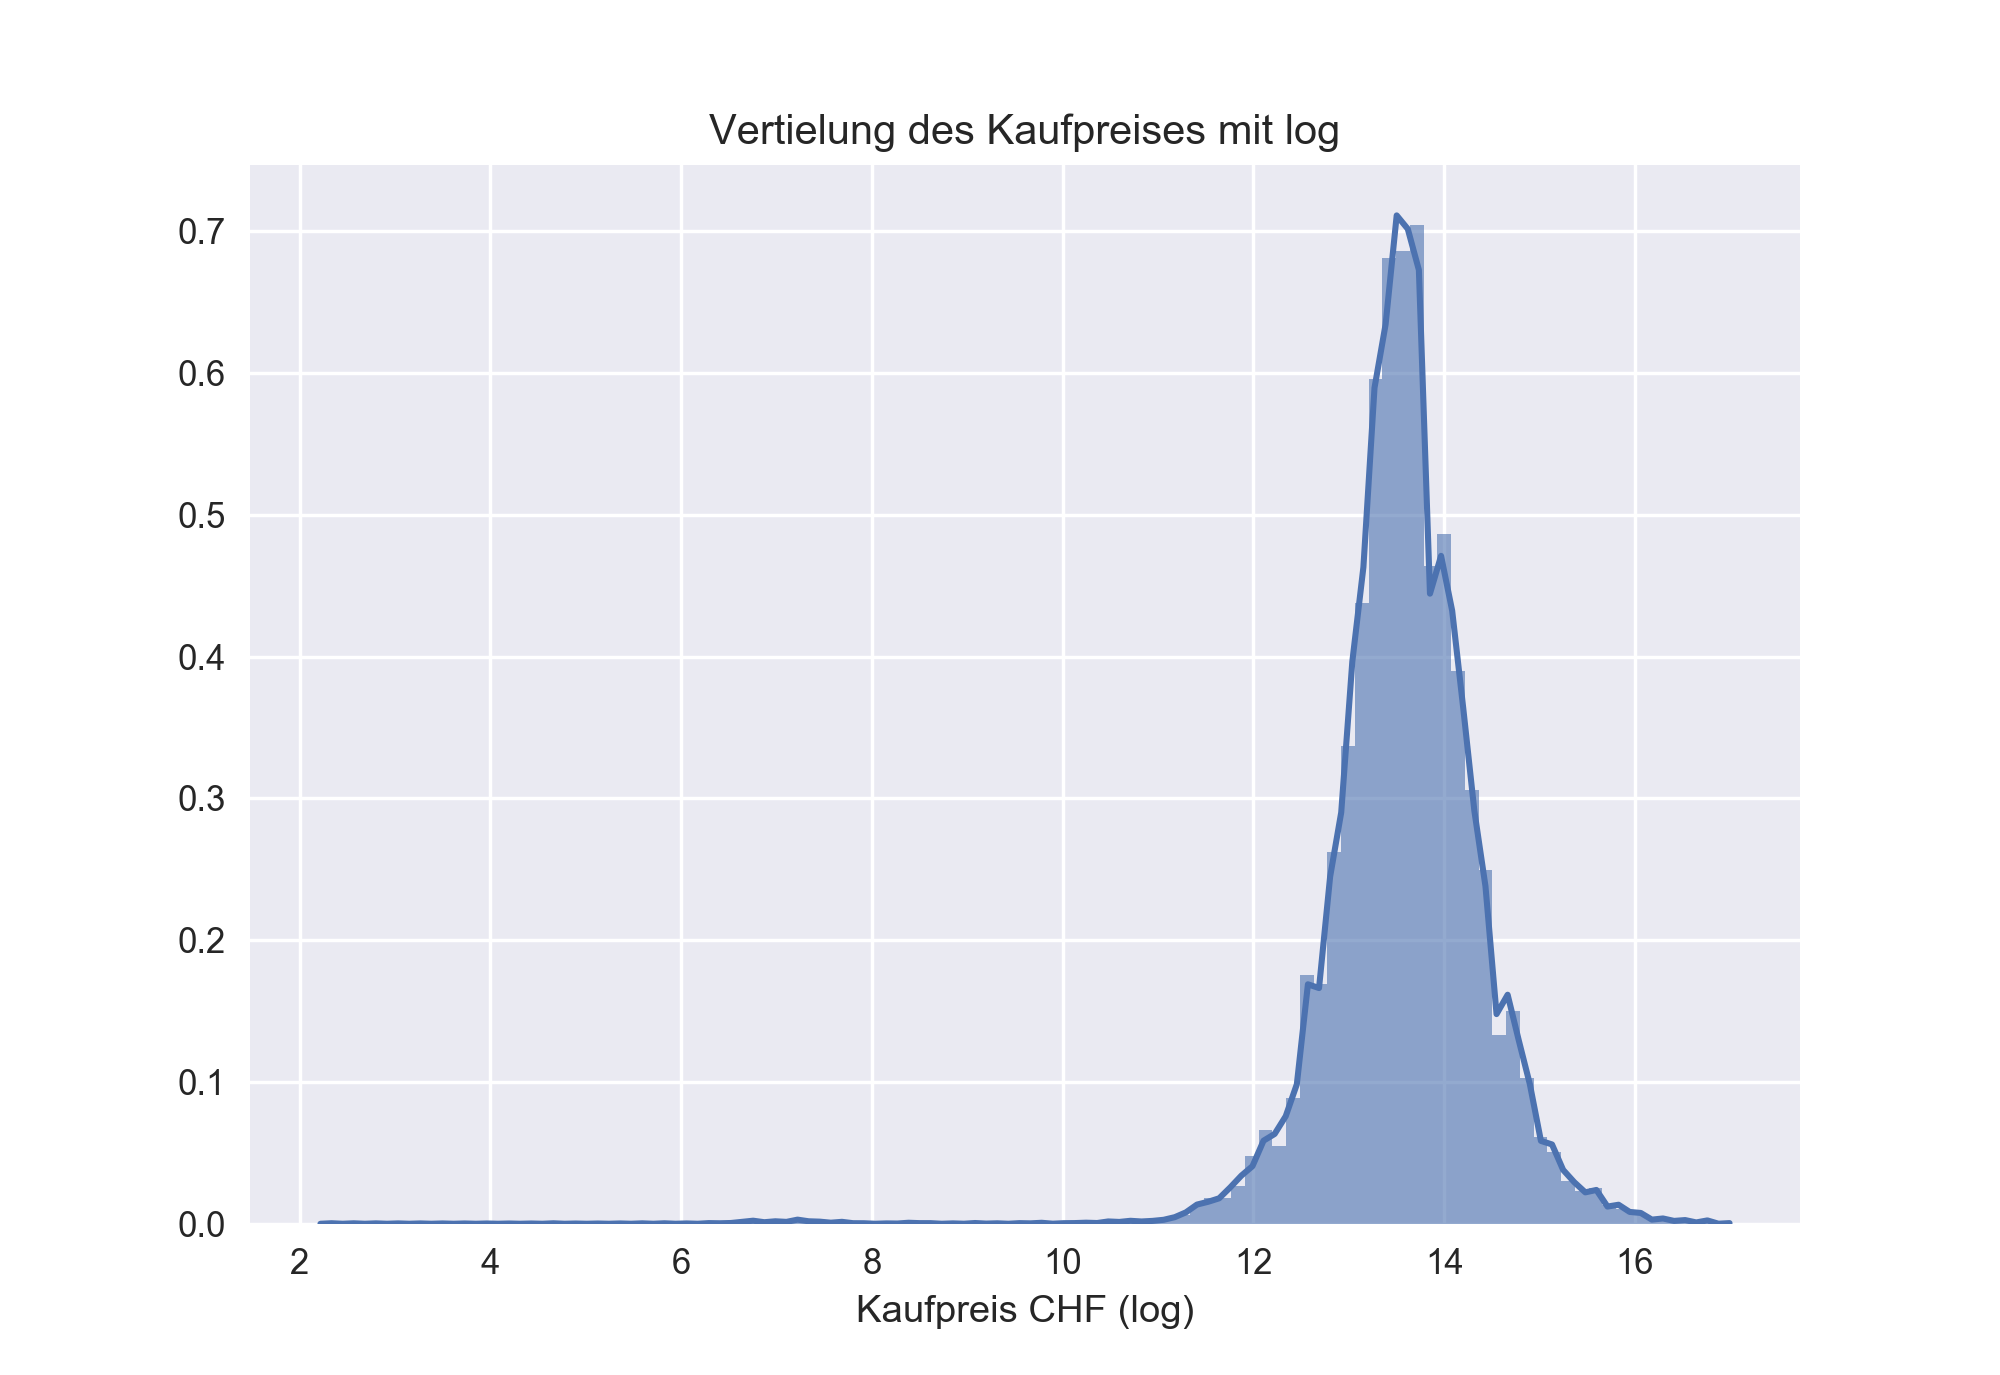
\includegraphics[width=\linewidth]{images/Verteilung_des_kauf_preises_log.png}
  \caption[Verteilung des Log(Preises)]{Verteilung des Log(Preises)}
  \label{fig:price_log}
\end{subfigure}
\caption[Kaufpreis analyse: Verteilung]{Kaufpreis analyse: Verteilung}
\label{fig:price}
\end{figure}
%
\begin{table*}[ht]
\centering
\ra{1.3}
\resizebox{\textwidth}{!}{
\begin{tabular}{@{}lrrrrr@{}}
\toprule
 & Min & Max & Durchschnitt & Median & Standardabweichung\\
\midrule
Preis: Haus & 10 & 20'000'000 & 1'281'735 & 920'000 & 1'309'085\\
Preis: Wohnung & 10 & 20'000'000 & 891’479 & 690’000 & 786’047\\
Pries: Alle & 10 & 20’000'000 & 1’059’503 & 790’000 & 1’066’372\\
\bottomrule
\end{tabular}}
\caption{Fehlermodelle mit Formelen}
\label{tab:error_models}
\end{table*}
%
\subsubsection{Numerische Features}
Bis auf die Lärmbelastung wurden alle numerischen Features von Inseraten gesammelt.\\
Abbildung \ref{fig:num_features} zeigt einen Teil dieser Features in Verbindung zum Kaufpreis. Dabei ist ersichtlich, dass die Wohnfläche, Kubatur und Anzahl Zimmer eine linear ähnliche Abhängigkeit haben. Beim Rest ist eher unklar, wie sie zum Preis stehen.\\[2ex]
%
\begin{figure}[h!]
\centering
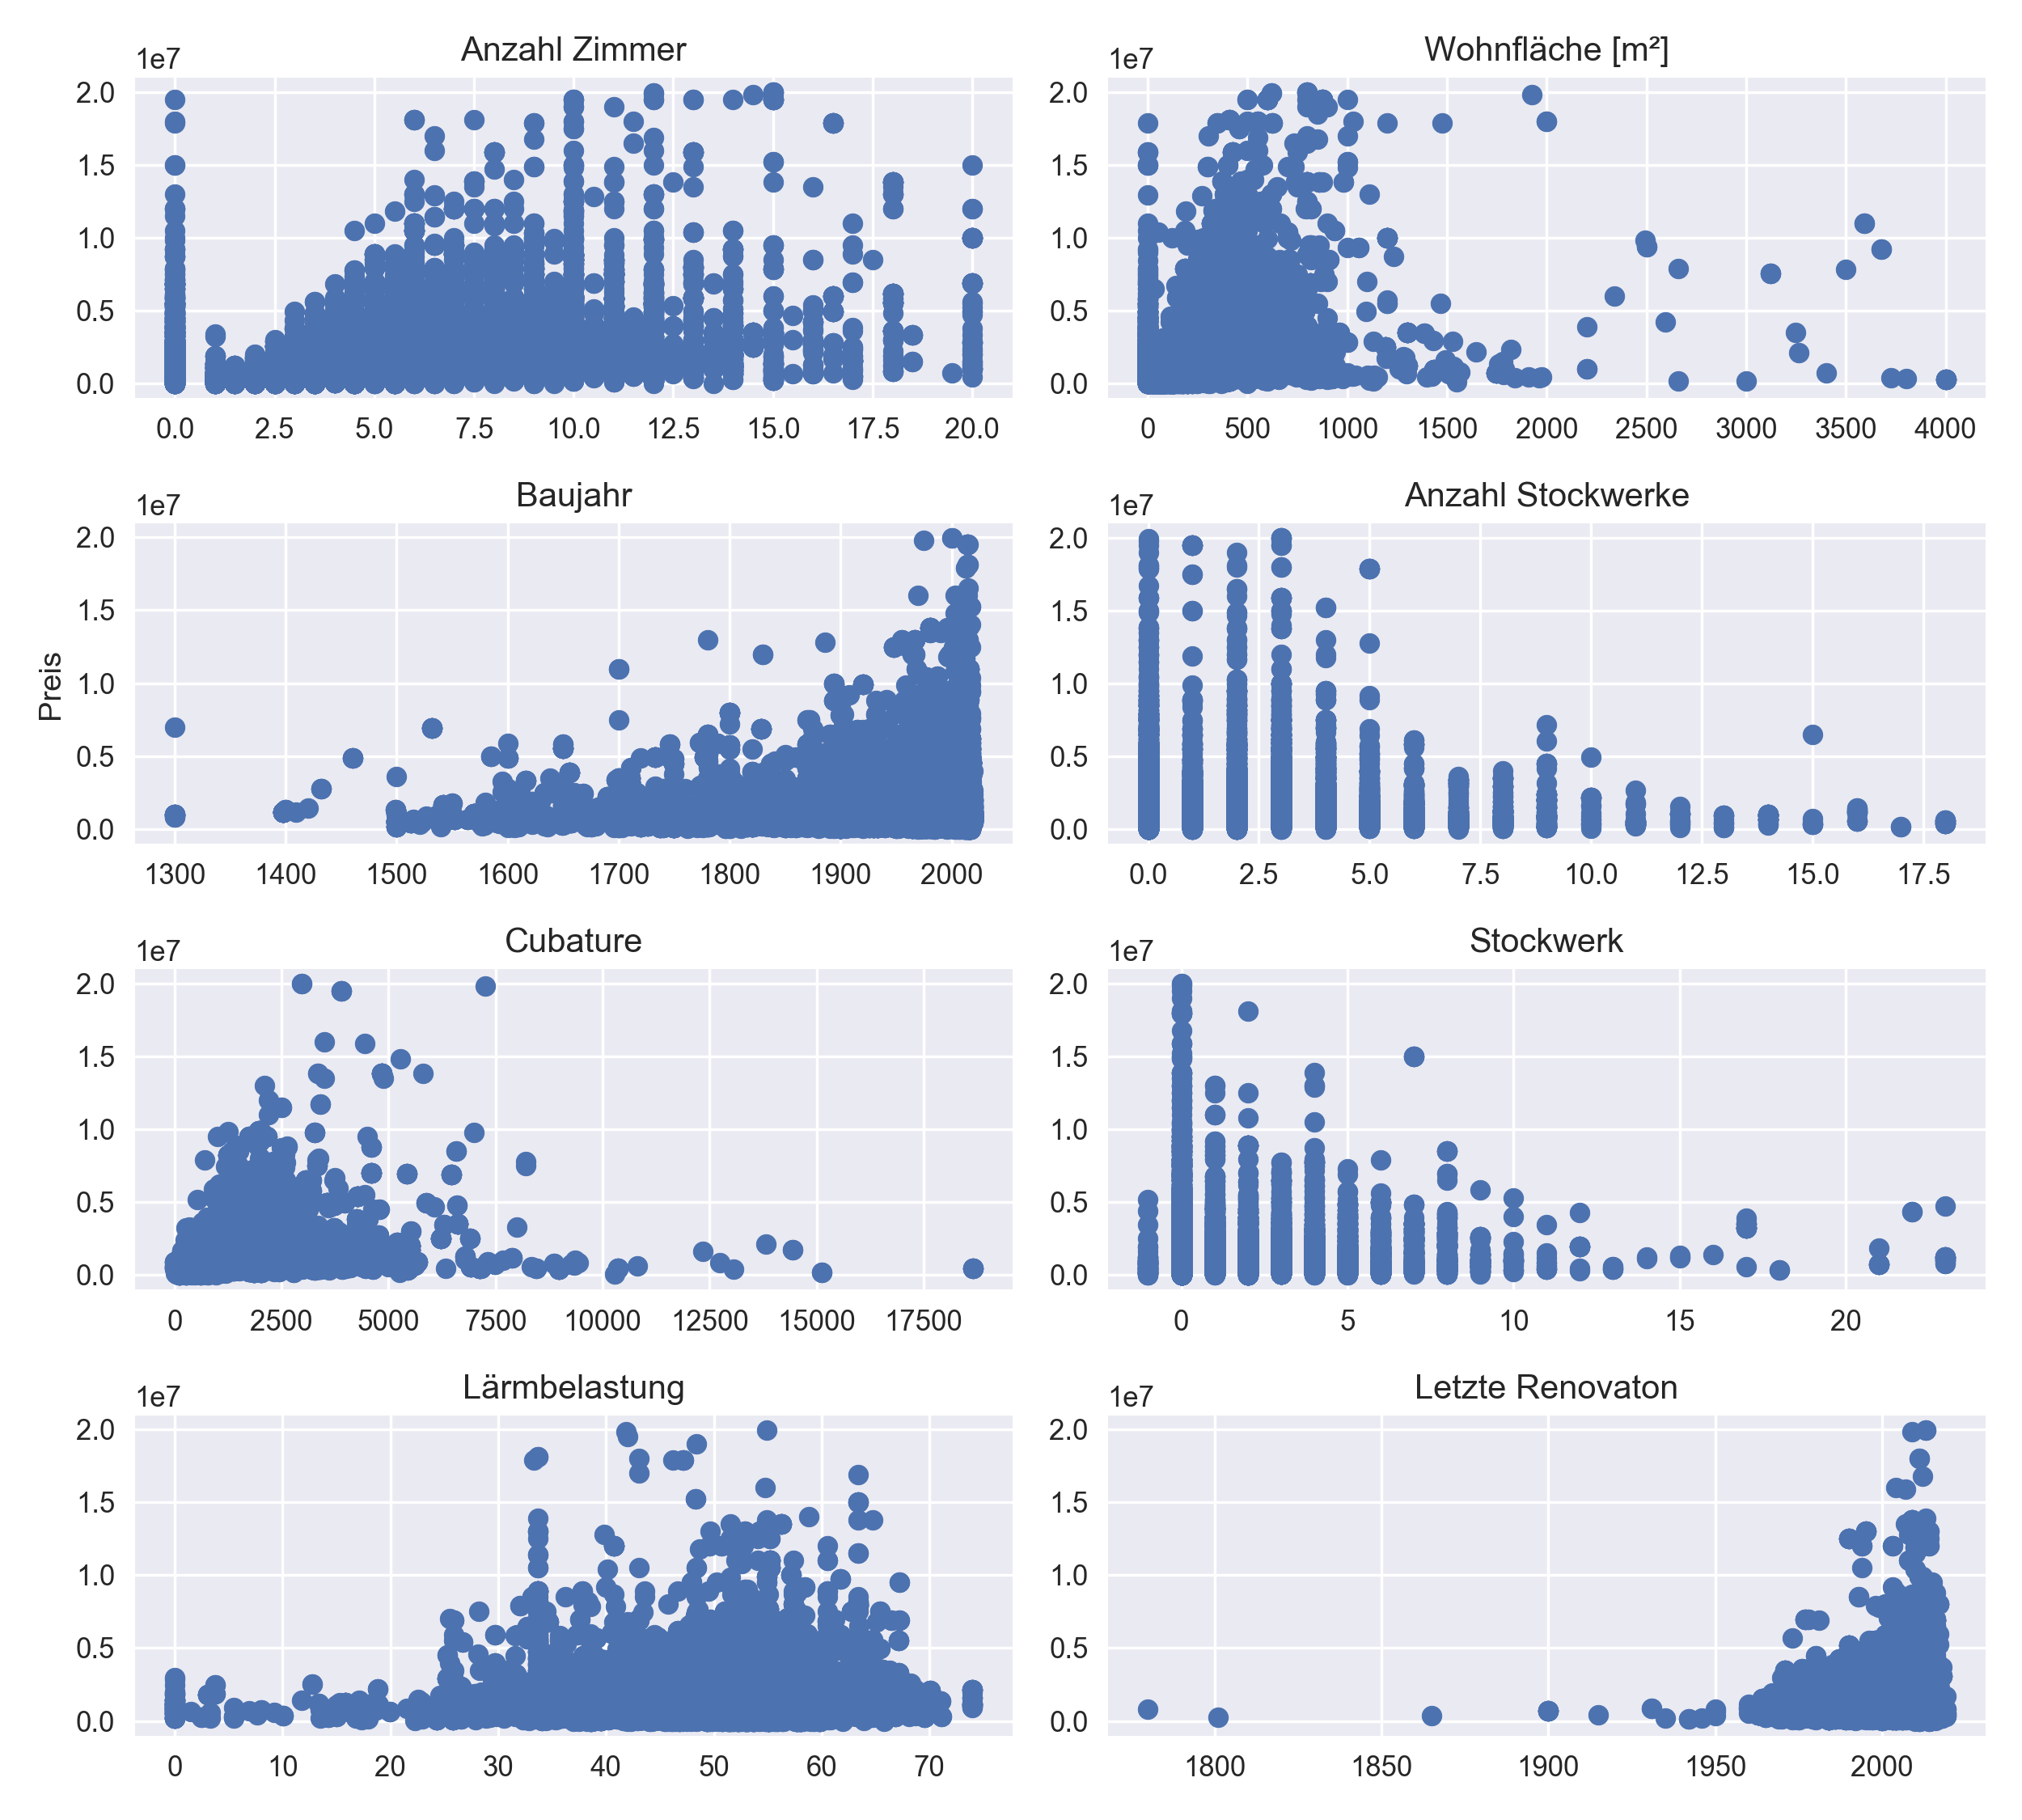
\includegraphics[width=0.9\textwidth]{images/Vergleich_zum_preis.png}
\caption[Nummerische Feature im Vergleich zum Preis]{Nummerische Feature im Vergleich zum Preis}%
\label{fig:num_features}
\end{figure}
\newline
%
Tabelle \ref{tab:num_features} zeigt die statistischen Werte für die numerischen Features. Die gesammelten Kennwerte sehen plausibel aus und decken sich zum Teil mit den Daten vom Bundesamt für Statistik\footnote{https://www.bfs.admin.ch/bfs/de/home/statistiken/bau-wohnungswesen.html}.\\
Auffallend ist, dass der Durchschnitt und der Median bei vielen Features sehr nahe beieinander liegen. Somit gleicht die Verteilung einer Normalverteilung.\\
Einzig störend sind die 0-Werte bei den Features Anzahl Zimmer und Fläche. Diese sollte wenn möglich weitgehend herausgefiltert werden.\\[2ex]
%
\begin{table*}[ht]
\centering
\ra{1.3}
\resizebox{\textwidth}{!}{
\begin{tabular}{@{}lrrrrr@{}}
\toprule
 & Min & Max & Durchschnitt & Median & Standardabweichung\\
\midrule
Anz. Zimmer & 0& 20 & 4.84 & 4.5 & 1.9\\
Fläche & 0 & 4’000 & 143.08 & 130 & 101.924\\
Baujahr & 1300 & 2019 & 1988 & 2006 & 51.52\\
Anz. Stockwerke & 0 & 18 & 1.8 & 2 & 1.747\\
Kubatur & 1 & 18649 & 1059.74 & 867 & 838.419\\
Stockwerk & -1 & 23 & 1.25 & 1 & 1.57\\
Lärmbelastung & 0 & 73.99 & 48.8 & 49.35 & 6.85\\
Letzte Renovation & 1780 & 2019 & 2009 & 2012 & 9.09\\
\bottomrule
\end{tabular}}
\caption{Statistische Werte der nummerischen Features}
\label{tab:num_features}
\end{table*}
%
Abbildung \ref{fig:heatmap} zeigt eine Heatmap der einzelnen Features. Sie zeigt, welche Features stark untereinander korrelieren. Folglich demonstriert sie von welchen Features der Preis abhängig ist. Somit sollte wenn möglich alle Features, die eine hohe Korrelation mit dem Kaufpreis besitzen, ins Modell miteinbezogen werden.
%
\begin{figure}[h!]
\centering
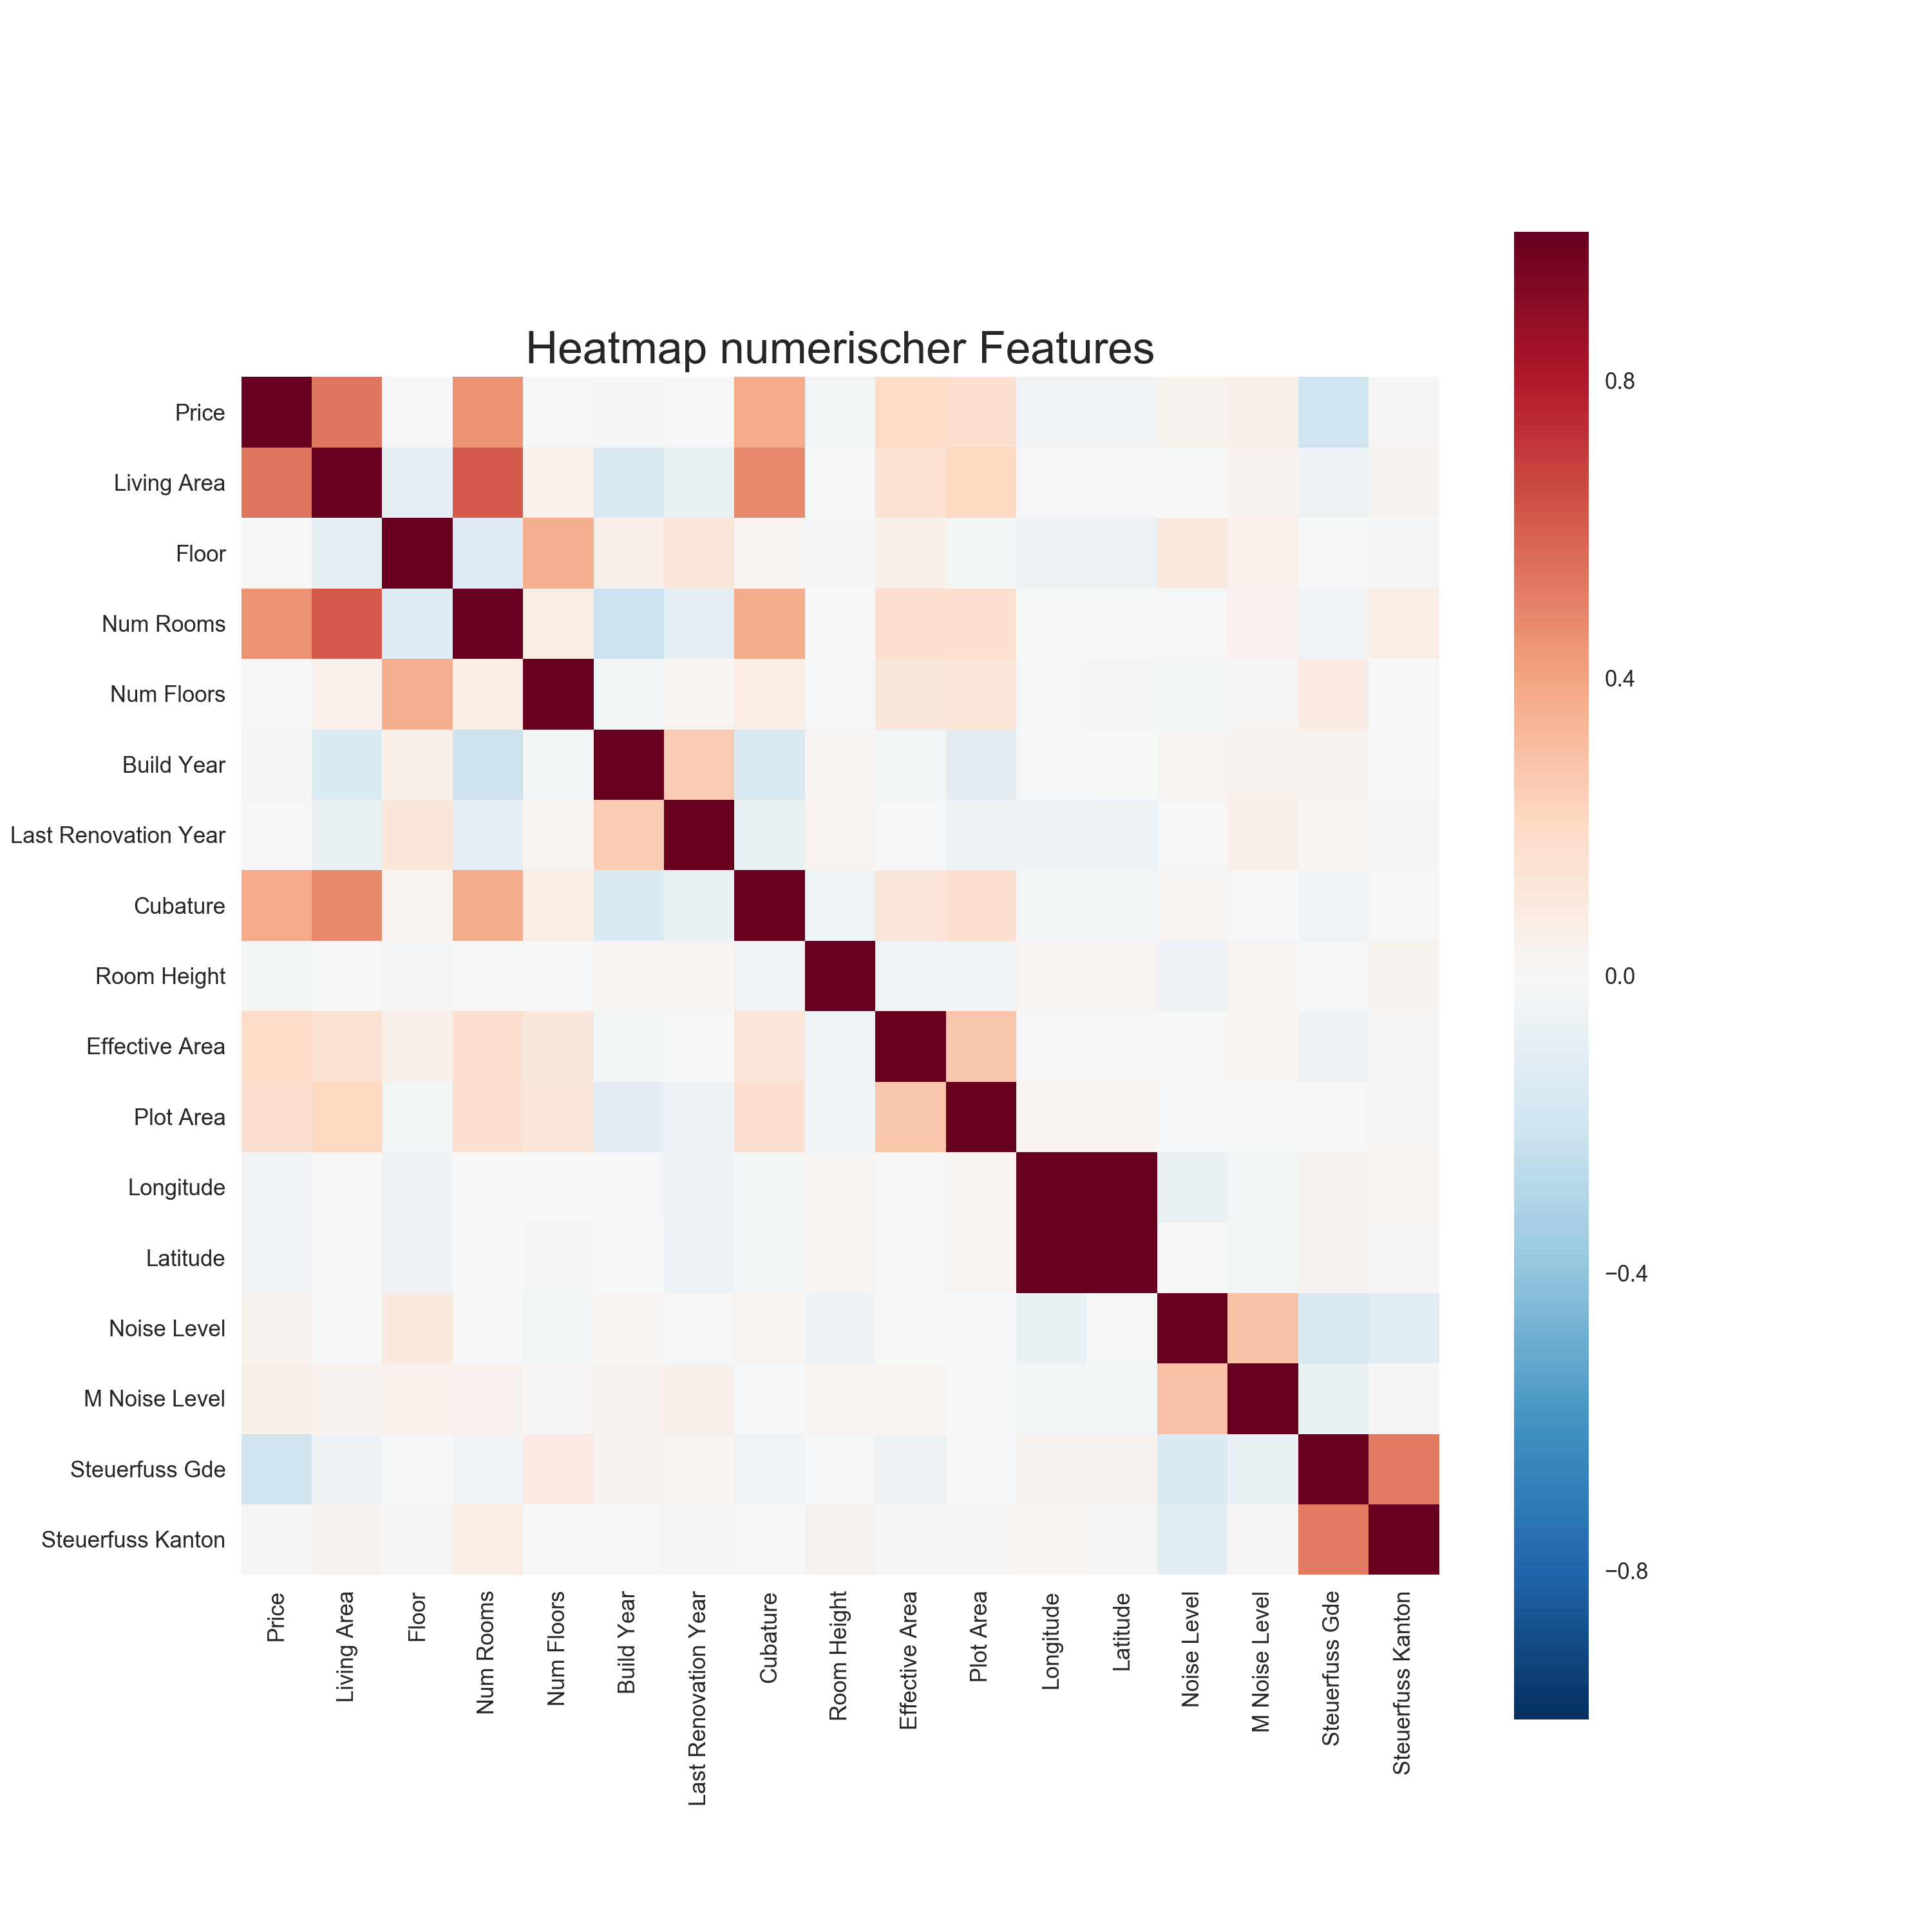
\includegraphics[width=0.9\textwidth]{images/Heatmap_numerical.png}
\caption[Heatmap der nummerischen Features]{Heatmap der nummerischen Features}%
\label{fig:heatmap}
\end{figure}
\newline
%
\subsubsection{Kategorische Features}
Bei den Kategorischen Features handelt es sich vor allem um ortsbezogene Features. Viele davon beschreiben die Region, indem sich die Immobilie befindet.\\
Insgesamt wurden 35 kategorische Features verwendet. Eine Analyse der ortsbezogenen Features mit dem Kaufpreis ergab keine unerwarteten Ergebnisse. So zeigt sich, dass der Kanton Genf die teuersten Immobilien in der Schweiz besitzt, gefolgt von Zug. Abbildung \ref{fig:cantons}.
Auch wurde ersichtlich, dass städtische Immobilien im Schnitt teurer sind als auf dem Land, beziehungsweise je urbaner die Region, desto teurer der Immobilienpreis. Weiter ist ersichtlich, dass  ein Haus im Schnitt mehr kostet als eine Wohnung.\\[2ex]
\begin{figure}[ht]
\centering
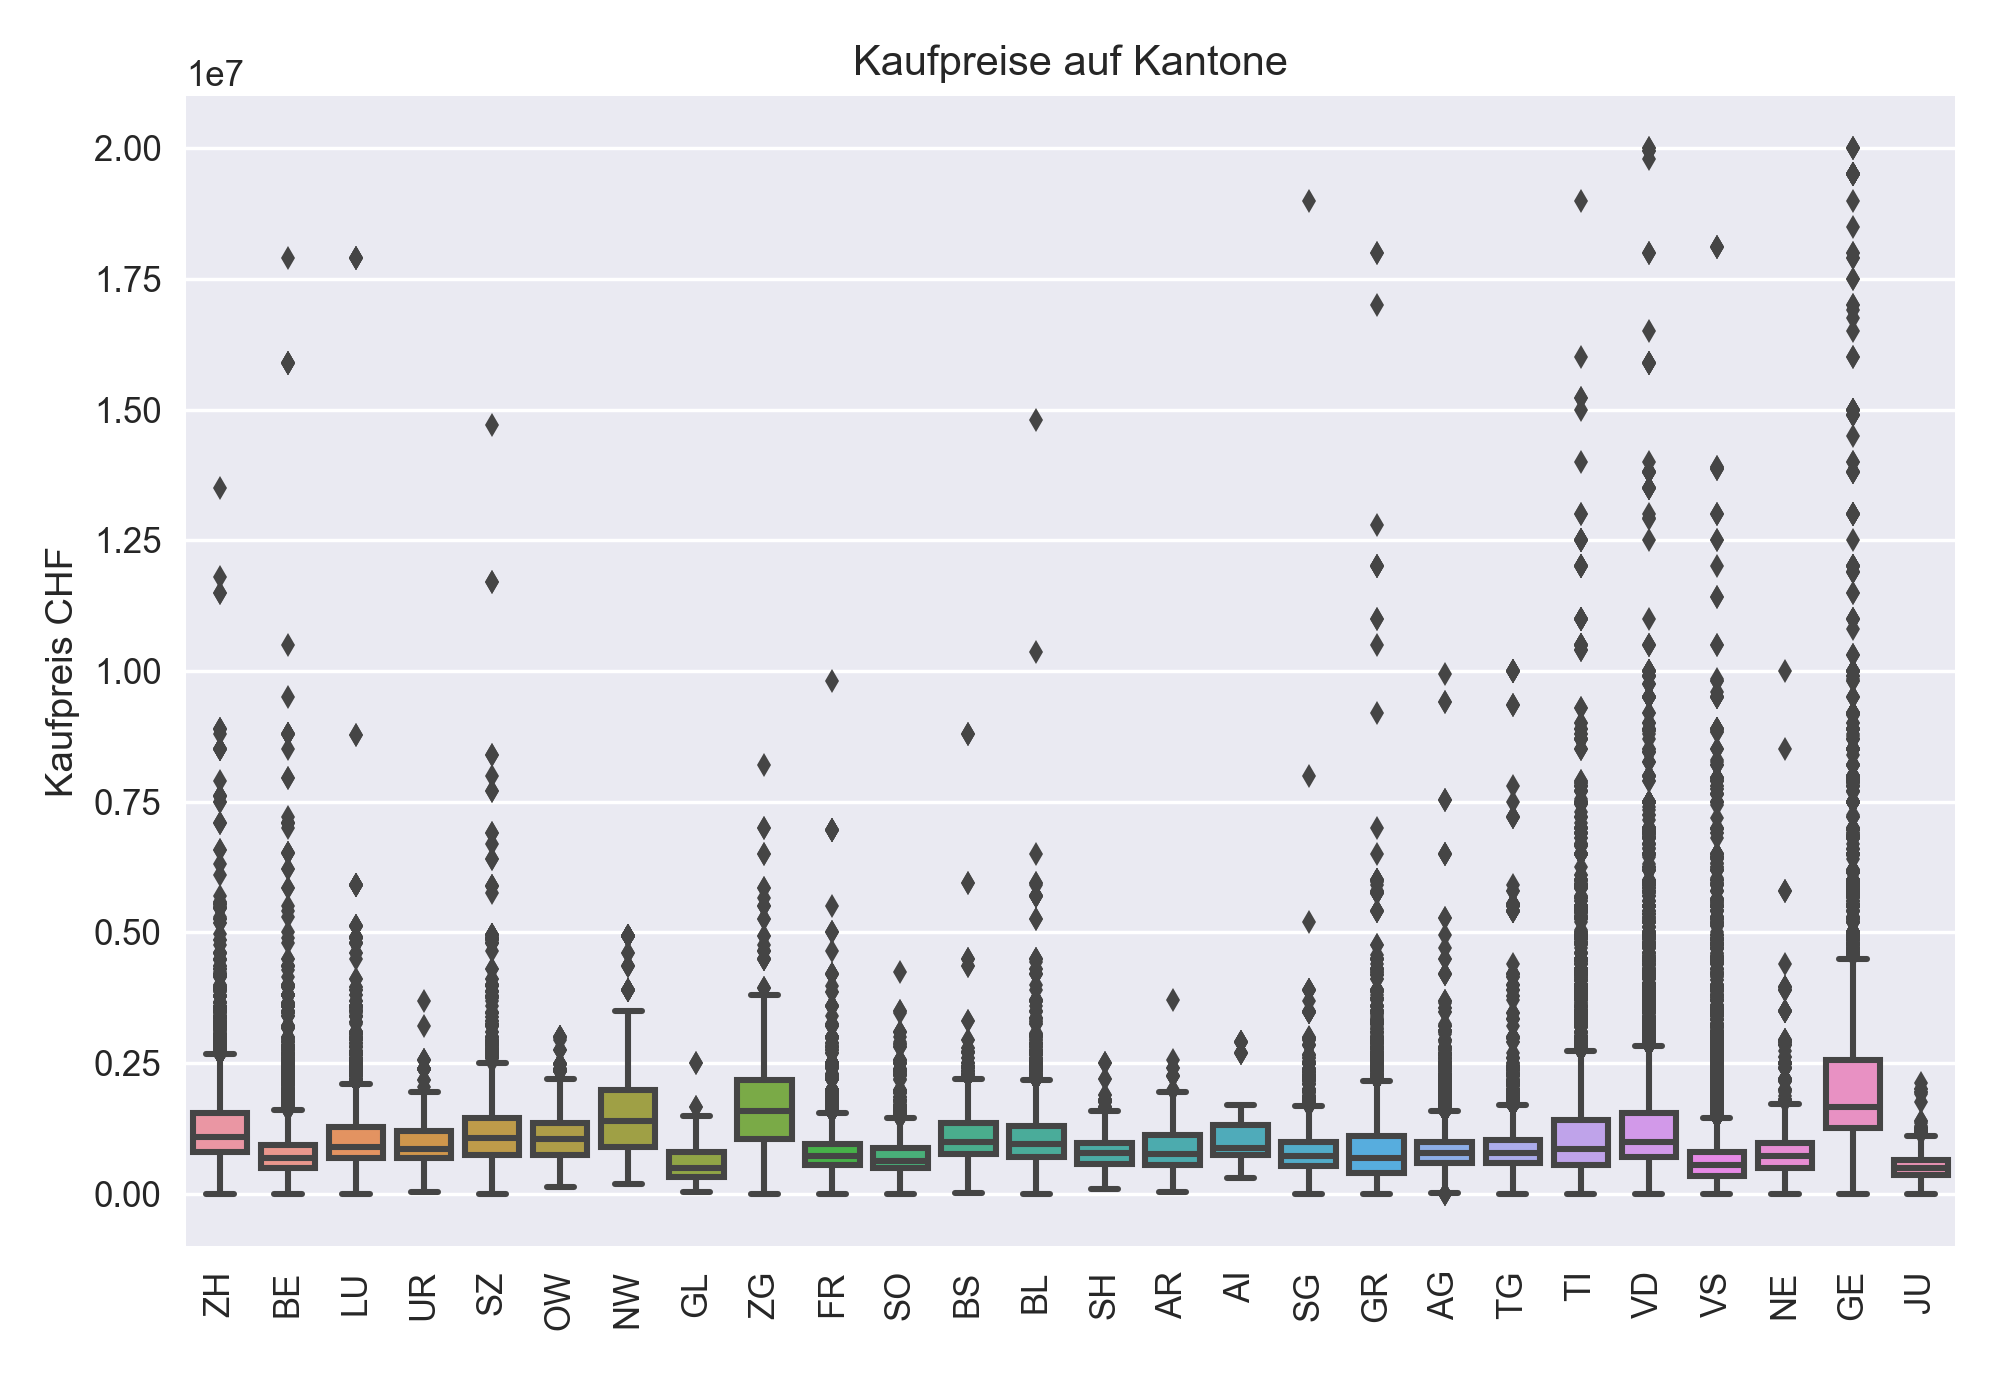
\includegraphics[width=\textwidth]{images/boxPlot_cantons.png}
\caption[Kaufpreis auf Kantonte aufgeteilt]{Kaufpreis auf Kantonte aufgeteilt}%
\label{fig:cantons}
\end{figure}
\newline
%
\textbf{Beschreibung / Charakteristik}
Weitere charakteristische Features stammen aus der Beschreibung und Merkmal analyse. Die 50 häufigsten vorkommenden Wörter die in unserem Datensatz vorkommen, werden in Abbildung \ref{fig:tags} gezeigt. 
\begin{figure}[ht]
\centering
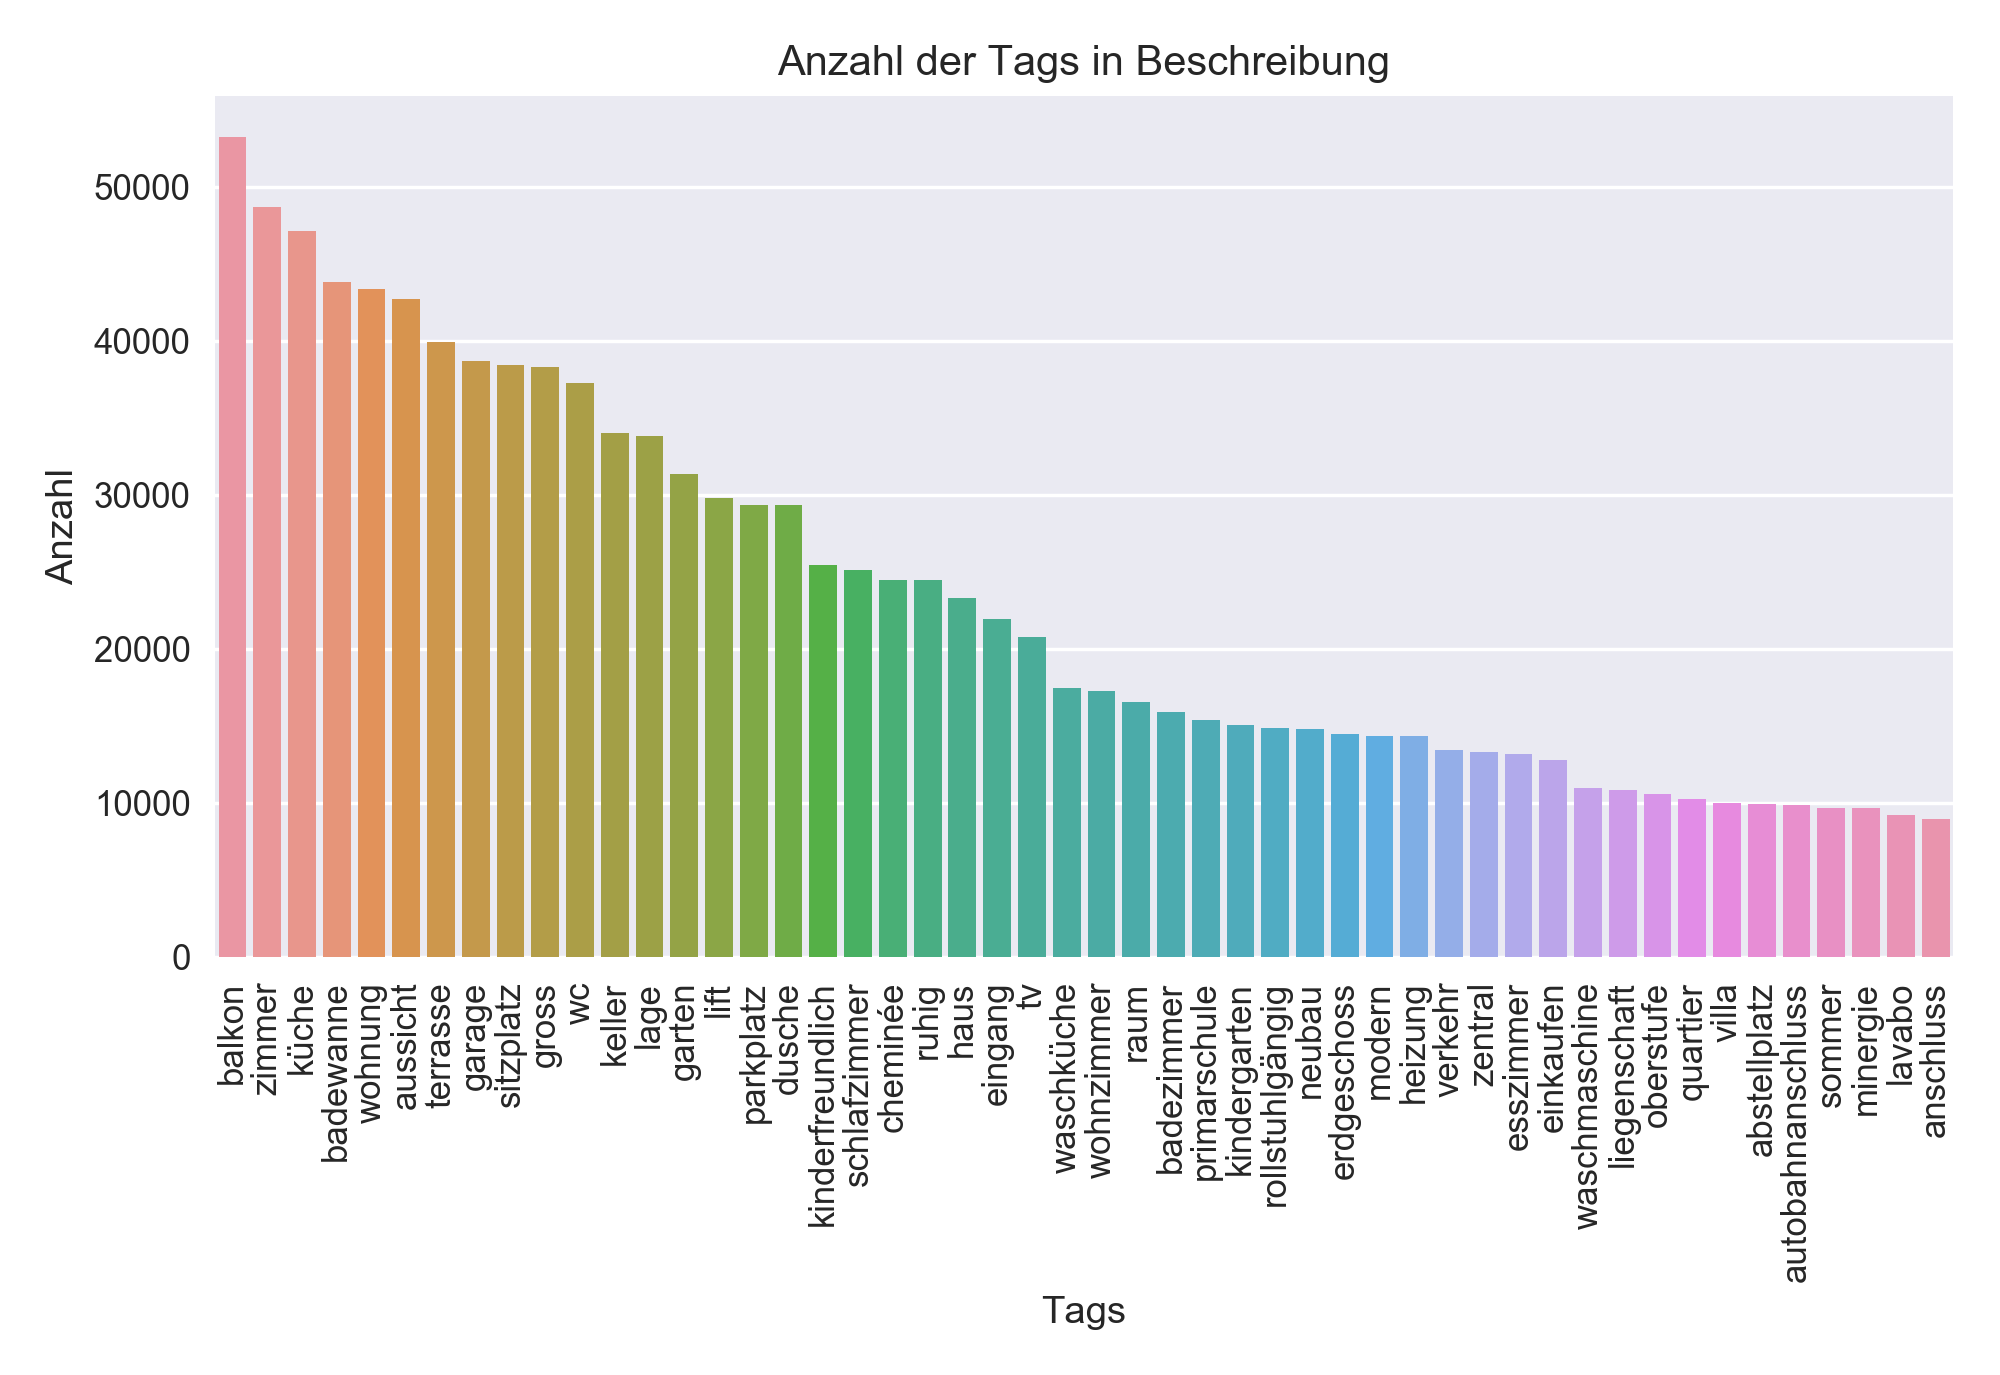
\includegraphics[width=\textwidth]{images/tags.png}
\caption[Häufigkeit der gefundenen Tags]{Häufigkeit der gefundenen Tags}%
\label{fig:tags}
\end{figure}
\newline
%
\subsection{Machine Learning}
Insgesamt haben wir neun verschiedene Machine Learning Algorithmen untersucht. Um eine faire Bewertung zu bekommen, bekamen alle Algorithmen die gleichen Datensätze zum Trainieren wie auch zum Testen. So wurde verhindert, dass ein Algorithmus anhand eines guten Datensatzes eine bessere Performance erzielte.\\[2ex]
%
Damit wir unsere gesammelten Daten für die Algorithmen verwenden können, müssen diese, wenn nötig, richtig transformiert werden. Dafür wird Feature Engineering angewendet, das nach und nach erweitert und verbessert wird.\\[2ex]
%
Als Basis für unsere Feature Engineering Pipeline transformieren wir unseren kategorischen Features mit Hilfe einer One-Hot-Encoding in binäre Features um. So konnten aus 35 Features über 2000 Features gewonnen werden.\\
Es ist nicht möglich alle gesammelten Features zu verwenden. Der Grund ist, dass gewisse Features nur bei wenigen Inseraten angegeben wurden. Wie im vorherigen Kapitel gezeigt, sind dies die Features Kubatur, Raumhöhe, effektive Fläche, Grundstücksfläche, Anzahl Stockwerke, Stockwerk und Renovationsjahr.\\
Als letzter Schritt werden die Inserate gelöscht, die keinen Eintrag bei einem verwendeten Feature besitzen oder doppelt vorkommen. Verwendet werden schlussendlich: Wohnfläche, Anzahl Zimmer, Baujahr Renovationsjahr, die Beschreibung und die Merkmale.\\[2ex]

Für die Auswertung der Algorithmen starten wir mit den Regressions Algorithmen. Hierfür verwenden wir: Lineare Regression, Ridge und der Lasso Algorithmus. Die Ergebnisse werden in Tabelle() angezeigt.



\newpage
\clearpage
%
\section{Diskussion}
In dieser Arbeit konnte erfolgreich aufgezeigt werden, dass anhand von öffentlichen Daten und modernen Machine Learning Methoden eine akkurate Schätzung abgeben werden kann.\\[2ex]
%
Das sammeln von öffentlichen Daten ist jedoch mit einem gewissen Aufwand verbunden. Die Datenqualität der verschiedenen Immobilienplattformen sind eher dürftig. Es konnten somit nur sehr wenige Kennwerte einer Immobilie verwendet werden. Bei einer professionellen Schätzung kämen noch diverse andere Kennwerte zum Einsatz.\\
Ist die Idee über längere Zeit Daten zu sammeln, lohnt es sich in einen autonomen Crawler Zeit zu investieren. So ist man nicht abhängig vom XPath oder CSS und ist gegenüber einem Redesign der Seiten gewappnet. Eine weitere Möglichkeit wäre die Daten bei einem vorhandenen Immobilienplattform direkt zu beziehen.\\
Die Verknüpfung der ortsbezogenen Daten mit den Inseraten kann zum Teil mühsam sein. Wir haben OpenStreetMap verwendet, um möglichst Kostengünstig die Koordinaten zu erhalten. Der Nachteil an OpenStreetMap ist, dass es mehrheitlich nur Städte abdeckt. Hier lohnt sich auf jeden Fall ein Konto bei Google Maps, da die Adresssuche viel besser ist.\\[2ex]
%
Das Crawlen über ein Proxy lohnt sich, da somit die Gefahr, als Crawler erkannt zu werden, verringert wird. Durch das wir über einen Server ausserhalb der Schweiz gingen, konnten wir nicht alle Plattformen, wie zum Beispiel Comparis, aufrufen.\\
Es ist eventuell sogar sinnvoll nur von einer Plattform die Daten zu sammeln. So müssen nicht die Unterschiedlichen Bezeichnungen harmonisiert werden.\\[2ex]
%
Das Untersuchen eines Machine Learning Algorithmus ist nicht immer einfach. Vor allem bei Baumalgorithmen. Denn die Teilung ist nicht immer gleich, auch wenn immer der gleiche Seed verwendet wird. So kann es sein, dass bei einem erneuten Durchlauf ein wenig bessere oder schlechtere Resultate herauskommen.\\
Zusätzlich muss beachtet werden, dass wir vor allem Standardimmobilien in unserem Datensatz haben. Sprich ausgefallene Inserate können nur schwer geschätzt werden, wenn sie nicht schon bei der Outlier Detection herausgenommen wurden. Somit eignen sich unsere Modell nicht für ausgefallene Immobilien.\\[2ex]
%
Aufgefallen ist uns auch, dass je mehr Inserate man verwendet desto besser wurden die Baumalgorithmen. Verwendeten wir nur die Hälfte der Inserate konnten die Modelle nur noch etwa 72\% Prozent mit einer Abweichung von 10\% richtig schätzen. Besitzt man weniger Inserate, könnte ein Baumalgorithmus nicht unbedingt am geeignesten sein. Hier lohnt es sich eventuell den K-Nearest Neighbour zu verwenden.
\\[2ex]
%
Unsere eigen aufgebautes Pipeline-System hat uns beim Iterativen Prozess sehr unterstützt. So konnte ohne grosse Mühe diverse Szenarien durchgerechnet werden, ohne dass dazwischen Daten verändert werden müssen.
%	
\subsection{Weiterführende Anwendung} 
Es gibt noch viele weitere Machine Learning Algorithmen, die man untersuchen könnte. Unter Anderem wäre der LightGBM wie auch Neurale Netzwerke interessant zu untersuchen.\\ 
Weiter können unsere Modelle für Immobilienmakler verwendet werden. Dazu müsste man eine Web-Applikation zur Verfügung stellen, bei dem die Kennwerte eingetragen werden können und der Preis geschätzt wird. 


\newpage
\clearpage
%
\section{Zusammenfassung}

\newpage
\clearpage
\addcontentsline{toc}{section}{Literatur}
% Literaturliste anzeigen
\bibliographystyle{ieeetr}
\bibliography{literatur}
%
\clearpage
\addcontentsline{toc}{section}{Abbildungen}
\listoffigures
%
\addcontentsline{toc}{section}{Tabellen}
\listoftables
%
\renewcommand{\lstlistlistingname}{Listingverzeichnis}
\newpage
\section{Anhang}
%
\end{document}
